
\chapter{Methods}

\section{Software System}

This section details the comprehensive software architecture of Medibot, highlighting the tools and technologies employed in the development of both the web interface and the mobile application. The system is designed to provide robust, scalable, and user-friendly platforms for patients and healthcare professionals, facilitating efficient symptom input, medical image uploads, and lab report sharing. 

\subsection{System Description}
Medibot is designed to bridge the gap between initial symptom analysis and professional healthcare guidance. It supports both patients and healthcare professionals in the context of diagnosis and decision-making.


\paragraph{Patient Perspective:}
\begin{itemize}
    \item \textbf{Symptom Input:} Patients engage with Medibot by providing descriptions of their symptoms either through natural language queries or structured interaction.
    \item \textbf{Image Upload:} Patients can upload medical images, such as X-rays, for integration into Medibot's diagnostic analysis.
    \item \textbf{Lab Report Sharing:} Patients can share existing lab reports, enhancing Medibot’s ability to contextualize and understand their health condition.
    \item \textbf{Preliminary Guidance:} Medibot provides initial diagnostic considerations, identifies areas of concern, and suggests appropriate medical specialties or next steps.
\end{itemize}

\paragraph{Healthcare Professional Perspective:}
\begin{itemize}
    \item \textbf{Consultative Resource:} Doctors and healthcare providers use Medibot as a supportive decision-making tool in their diagnostic processes.
    \item \textbf{Patient Contextualization:} Medibot offers insights derived from patient-reported symptoms, uploaded images, and lab reports, aiding healthcare professionals in assessments.
    \item \textbf{Efficiency Tool:} Medibot helps streamline the analysis of initial symptoms and identification of potential conditions, assisting doctors in triaging and managing cases more effectively.
\end{itemize}

\paragraph{Important Notes:}
\begin{itemize}
    \item \textbf{Direct Communication:} Medibot does not enable direct data exchange or communication between patients and doctors.
    \item \textbf{Emphasis on Support:} Medibot serves as an assistive tool, not a replacement for professional medical diagnosis.
\end{itemize}

\begin{figure}[H]  % Use the [H] specifier to place the figure exactly at this point in the text
    \centering
    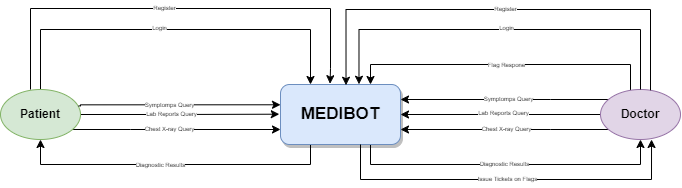
\includegraphics[width=0.8\textwidth]{./Figures/System Context.png}
    \caption{System Context Diagram}
    \label{fig:mysvg}
\end{figure}


\subsection{System Boundaries}

The Medibot system establishes well-defined boundaries to encapsulate its essential features and interactions with the external environment.
\subsubsection{Core components within the System}

\begin{itemize}
\item \textbf{Natural Language Processing (NLP) Engine:}
    \begin{itemize}
        \item Analyzes patient-provided symptom descriptions (text or potentially voice in the future).
        \item Processes medical text from lab reports.
        \item Generates preliminary diagnoses and potential health concerns.
    \end{itemize}

\item \textbf{Computer Vision (CV) Models:}
    \begin{itemize}
        \item Analyze uploaded medical images (e.g., X-rays) for abnormalities.
        \item May segment areas of interest (e.g., heart, lungs). 
    \end{itemize}

\item \textbf{Referral System:}
    \begin{itemize}  
       \item Matches potential diagnoses/concerns with relevant medical specialties.
       \item Provides guidance on appropriate next steps (e.g., specialist consultation, further testing).
    \end{itemize}    

\item \textbf{Knowledge Base:}
    \begin{itemize}
        \item Curated repository of medical information and diagnostic criteria.
        \item Supports inference and recommendations across the other components.
        \item Incorporates Retrieval-Augmented Generation (RAG) systems that enhance the AI's response capabilities by fetching relevant data and documents dynamically during the inference process.

    \end{itemize}

\end{itemize} % End of core components

\subsubsection{Interface Components within the System}

\begin{itemize}
    \item \textbf{Mobile Application:}
        \begin{itemize}
            \item User-friendly design optimized for smaller screens.
            \item Handles symptom input, image uploads, and output display.
            \item Built in apk format for Android devices.
        \end{itemize}

    \item \textbf{Web Application:}
        \begin{itemize}
            \item Offers a more expansive input area for larger text descriptions.
            \item Might handle large image uploads more efficiently.
            \item Built in a user-friendly web interface format.
        \end{itemize}
\end{itemize}

\subsubsection{Key Points at the Boundaries}

\begin{itemize}
    \item \textbf{Patient Inputs:}
        \begin{itemize}
            \item Direct symptom descriptions.
            \item Xray Image uploads.
            \item Sharing existing lab reports as Images.
        \end{itemize}

    \item \textbf{Medibot Outputs:}
        \begin{itemize}
            \item Preliminary diagnoses or highlighted concerns.
            \item Guidance and recommendations for follow-up actions.
            \item Referral suggestions to medical specialties.
        \end{itemize}

    \item \textbf{Interactions with Healthcare Professionals:} 
        \begin{itemize}
            \item Doctors may refer to Medibot's analyses as supplementary information during assessment (not primary data exchange).
        \end{itemize}
\end{itemize}

\subsubsection{Outside System Boundaries}

\begin{itemize}
    \item \textbf{Direct Patient-Doctor Communication:} Medibot does not facilitate direct messaging or real-time consultations.
    \item \textbf{Appointment Scheduling:} Integration with hospital systems for booking appointments is currently out of scope.
    \item \textbf{Treatment Prescriptions:} Medibot avoids generating explicit treatment plans or medication recommendations.
    \item \textbf{Emergency Situations:} Medibot is not designed to replace qualified emergency medical assistance. 
\end{itemize}


\subsection{Objectives and Requirements} 


\subsubsection{Objectives}

The Medibot AI Assistant aims to fulfill the following core objectives:
\begin{itemize}
    \item \textbf{Accurate Medical Guidance:}  Provide reliable medical advice grounded in the analysis of user-reported symptoms.
    \item \textbf{Streamlined Referrals:}  Facilitate effective patient navigation by suggesting appropriate healthcare professionals or relevant medical departments. 
    \item \textbf{Enhanced User Experience:} Deliver a seamless and intuitive experience for users throughout their interaction with the system.
\end{itemize}


\subsubsection{Requirements}

To meet these objectives, Medibot must satisfy the following user-driven requirements:

\begin{itemize}
    \item \textbf{Natural Language Input:} Enable users to describe their symptoms using everyday language, allowing for greater flexibility and comfort.
    \item \textbf{Timely and Relevant Advice:} Provide prompt responses with medical advice tailored to the user's reported symptoms and concerns.
\end{itemize}

\subsubsection{Desired Characteristics}
Beyond  requirements,  Medibot  strives  to  attain the following characteristics that reinforce its  value as an assistive tool:

\begin{itemize}
    \item \textbf{Accuracy:}  Consistently provide dependable advice through the utilization of robust models and up-to-date medical knowledge.
    \item \textbf{Reliability:} Deliver a steady and predictable user experience, promoting trust.
    \item \textbf{User-friendliness:} Craft an intuitive interface that guides inexperienced users throughout their interaction with the system.
\end{itemize}


\subsection{System Requirements}

\subsubsection{Use Case Diagram}
\begin{figure}[H] 
    \centering
    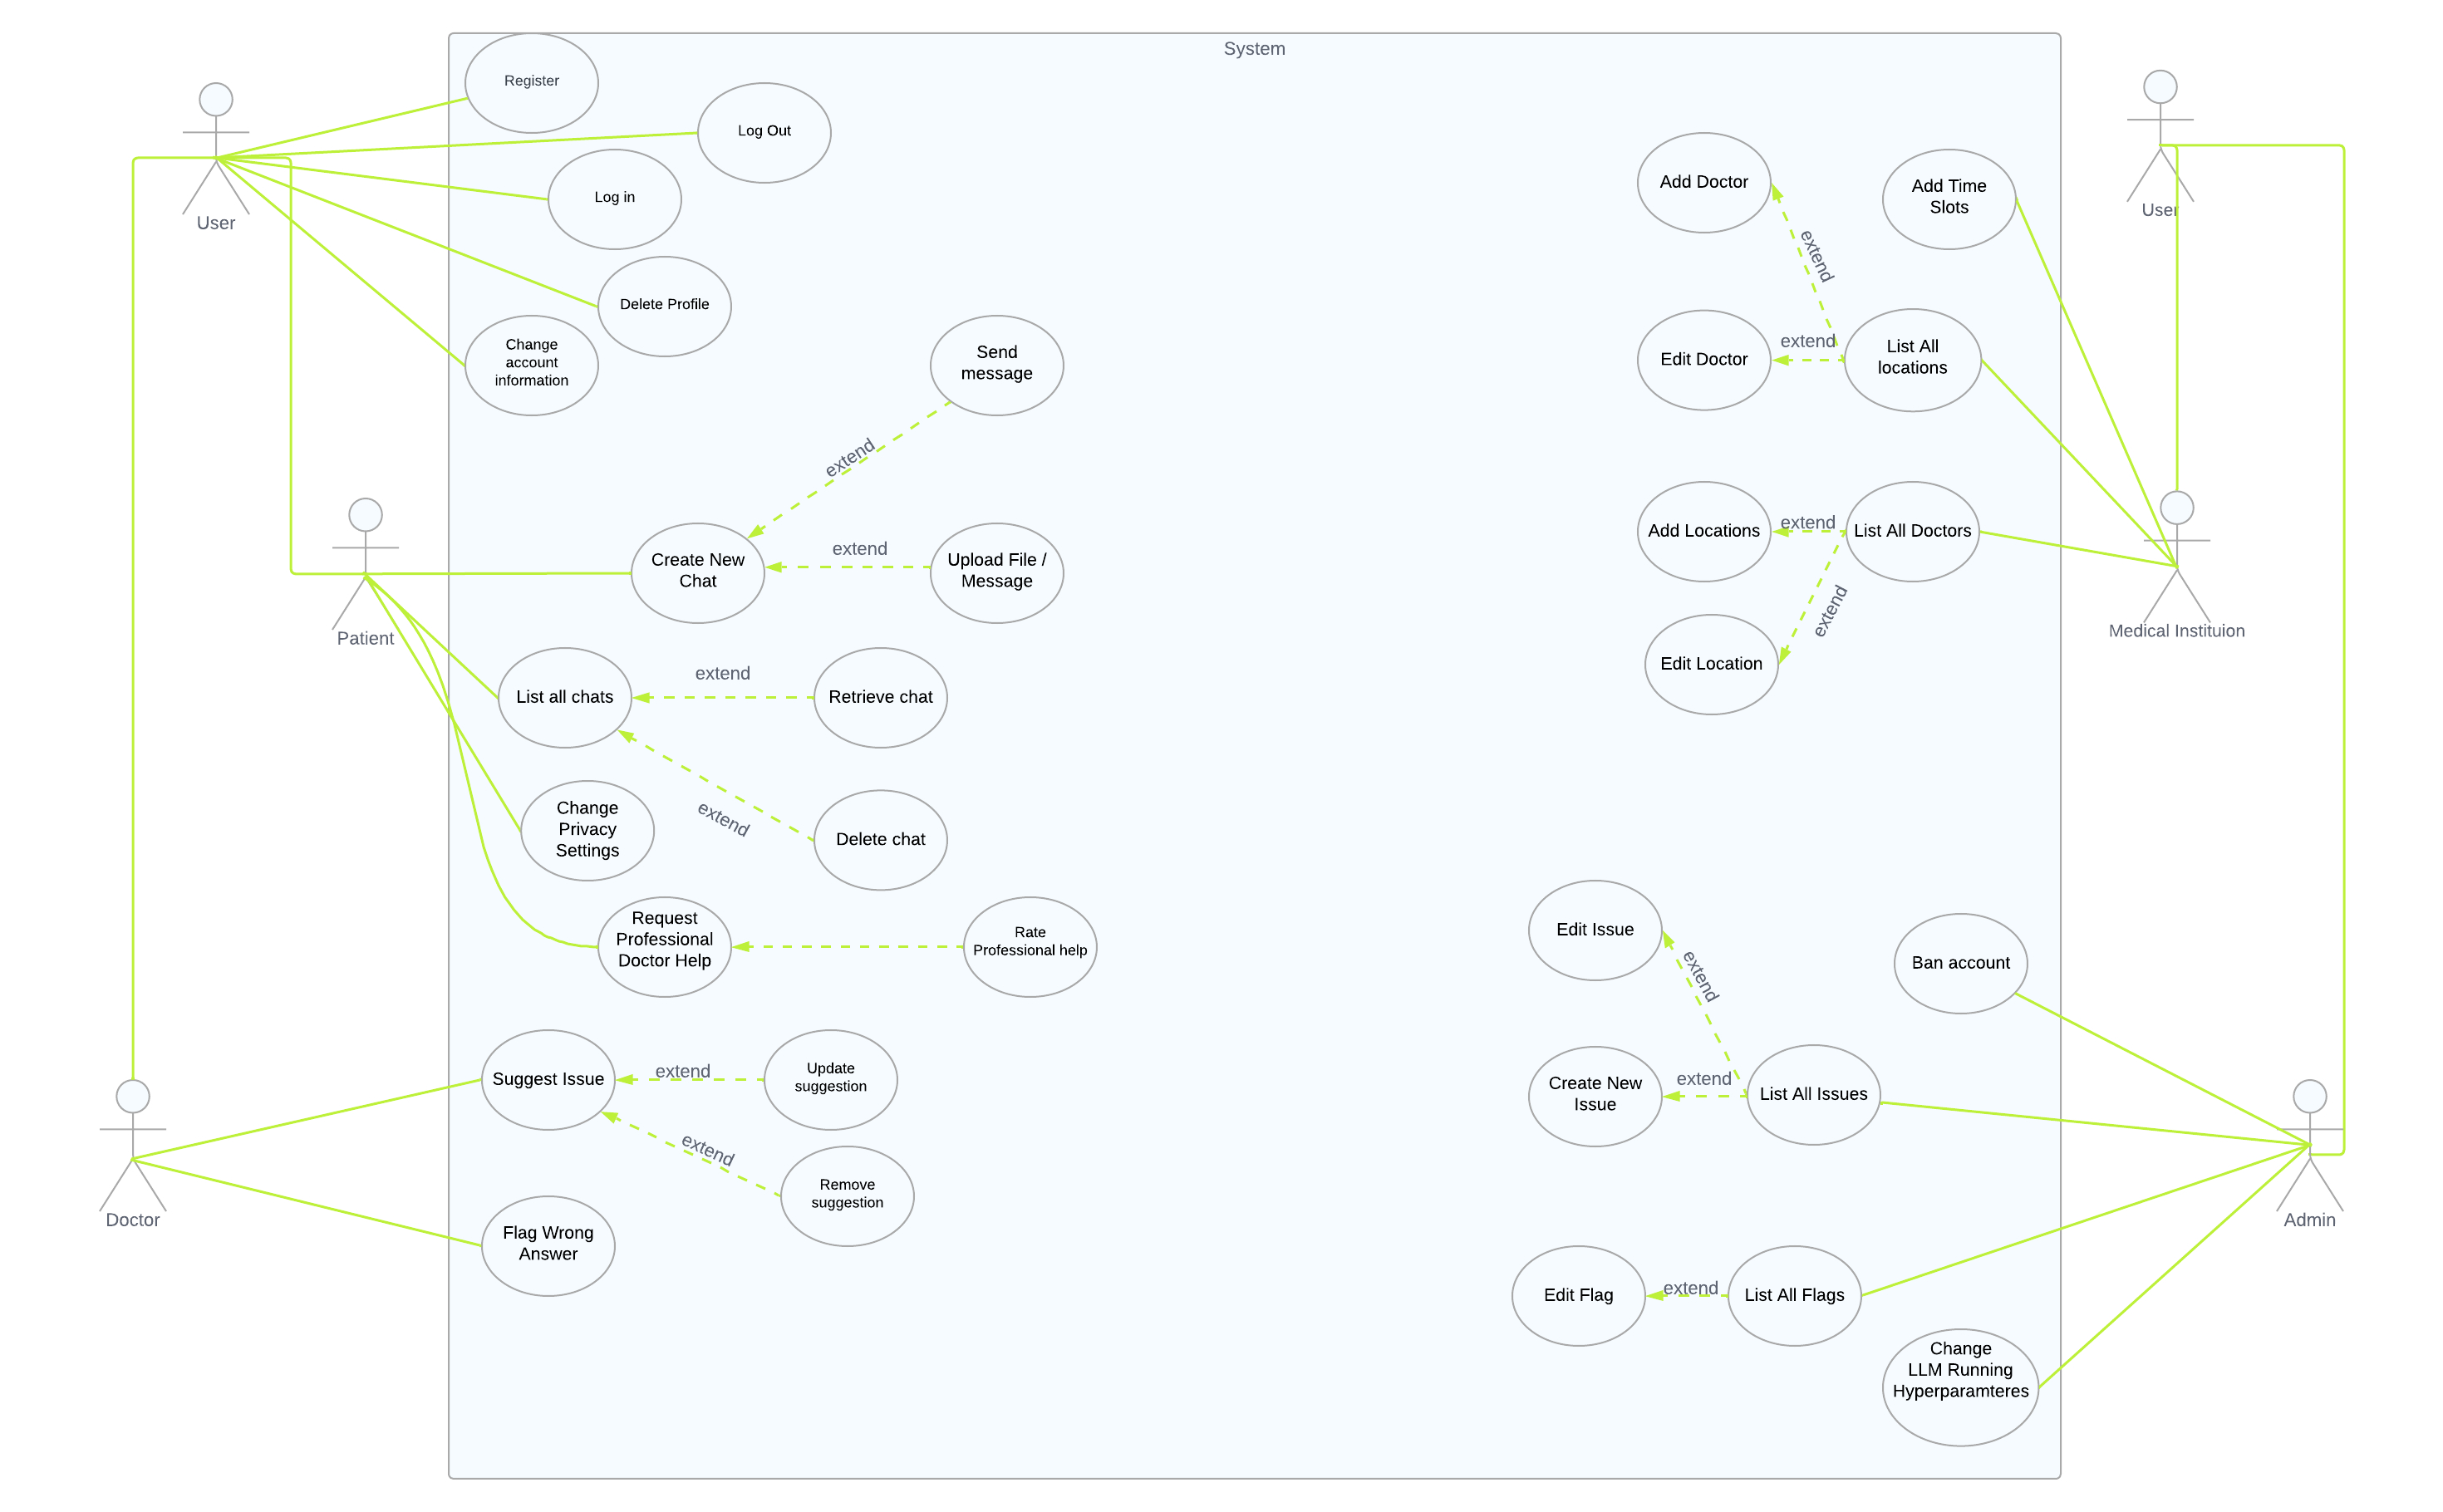
\includegraphics[width=0.8\textwidth]{./Figures/use_case.jpg} 
    \caption{System Context Diagram} 
    \label{fig:mysvg} 
\end{figure}


\subsubsection{General Functionality}
Medibot enables users to input symptoms, receive medical advice, and obtain referrals to appropriate healthcare professionals or departments. Project requirements include symptom analysis, integration with medical databases for diagnosis prediction, and seamless communication with users through text.

\subsubsection{Software Interfaces}
The system interfaces with users through both an Android mobile application and a Website. These user-friendly interfaces allow users to input symptoms and receive medical advice. Additionally, the system interacts with medical databases for accessing patient records and diagnostic information.

\subsubsection{Application Programming Interface (API)}
Medibot uses API to integrate its functionalities across all its modules in a single interface. The API includes functions for symptom analysis, diagnosis prediction, and image processing.

\begin{figure}[H] 
    \centering
    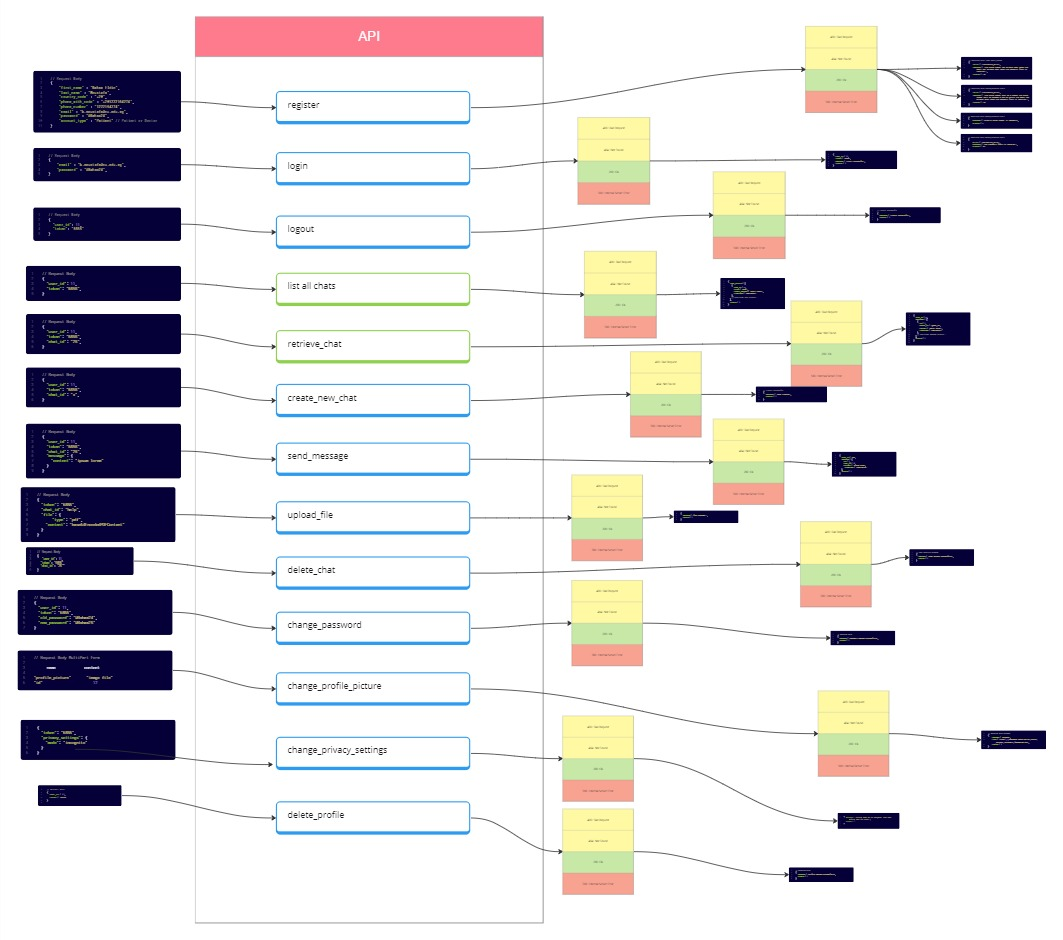
\includegraphics[width=0.8\textwidth]{./Figures/api.jpg} 
    \caption{API Endpoints} 
    \label{fig:mysvg2}
\end{figure}

\subsubsection{Functional Requirements}
\textbf{FR 1: Register}
\begin{itemize}
    \item \textbf{Actors:} Patient or Doctor
    \item \textbf{Description:} The system shall allow users (both students and instructors) to create accounts. The registration process shall securely collect the following information: username, password, and other required details. 
\end{itemize} 

\textbf{FR 2: Login} 
\begin{itemize}
    \item \textbf{Actors:} Patient or Doctor
    \item \textbf{Description:} Users shall be able to log in to the system using their registered credentials.
\end{itemize}

\textbf{FR 3: Logout} 
\begin{itemize}
    \item \textbf{Actors:} Patient or Doctor
    \item \textbf{Description:} Users shall be able to log out of their current session securely.
\end{itemize}

\textbf{FR 4: Create New Chat}
\begin{itemize}
    \item \textbf{Actors:} Patient or Doctor
    \item \textbf{Description:} Users shall be able to initiate new chat conversations.
\end{itemize}

\textbf{FR 5: Send Message}  
\begin{itemize}
    \item \textbf{Actors:} Patient or Doctor
    \item \textbf{Description:} Users shall be able to send text messages within an active chat conversation.
\end{itemize}

\textbf{FR 6: Retrieve Chat} 
\begin{itemize}
    \item \textbf{Actors:} Patient or Doctor
    \item \textbf{Description:} Users shall be able to view existing chat conversations. 
\end{itemize}

\textbf{FR 7: List All Chats}
\begin{itemize}
    \item \textbf{Actors:} Patient or Doctor
    \item \textbf{Description:} Users shall be able to view a list of their active and/or past chat conversations.
\end{itemize} 


\textbf{FR 8: Upload X-ray Image} 
\begin{itemize}
    \item \textbf{Actors:} Patient or Doctor
    \item \textbf{Description:} Users shall be able to upload medical X-ray images for analysis.
\end{itemize}

\textbf{FR 9: Upload Lab Report Image} 
\begin{itemize}
    \item \textbf{Actors:} Patient or Doctor
    \item \textbf{Description:} Users shall be able to upload medical images of lab reports for analysis.
\end{itemize}

\textbf{FR 10: Upload Lab Report PDF} 
\begin{itemize}
    \item \textbf{Actors:} Patient or Doctor
    \item \textbf{Description:} Users shall be able to upload medical files of lab reports for analysis.
\end{itemize}


\textbf{FR 11: Change Password}
\begin{itemize}
    \item \textbf{Actors:} Patient or Doctor
    \item \textbf{Description:} Users shall be able to securely update their account password. 
\end{itemize}

\textbf{FR 12: Change Email}
\begin{itemize}
    \item \textbf{Actors:} Patient or Doctor
    \item \textbf{Description:} Users shall be able to modify their registered email address.
\end{itemize}

\textbf{FR 13: Delete Chat} 
\begin{itemize}
    \item \textbf{Actors:} Patient or Doctor
    \item \textbf{Description:}  Users shall have the ability to delete specific chat conversations from their history.
\end{itemize}

\textbf{FR 14: Delete Profile} 
\begin{itemize}
    \item \textbf{Actors:} Patient or Doctor
    \item \textbf{Description:} Users shall have the ability to permanently delete their account and associated data from the system.
\end{itemize} 


\subsubsection{Non-Functional Requirements}

\textbf{Performance}


\begin{itemize}
    \item \textbf{NFR 1: Response Time}
        \begin{itemize}
            \item \textbf{Description:} Medibot shall generate preliminary diagnoses within 5 seconds of symptom submission for 90\% of user queries.
            \item \textbf{Priority:} High 
            \item \textbf{Metrics:} Measure average and percentiles (90th, 95th) of response time in testing and under varying load conditions.
        \end{itemize}

    \item \textbf{NFR 2: Image Upload and Processing} 
        \begin{itemize}
            \item \textbf{Description:}  Uploaded medical images (within permissible file size restrictions) should be processed for analysis within 30 seconds.
            \item \textbf{Priority:} Medium
            \item \textbf{Metrics:}  Track average and worst-case processing time, especially for large or complex image types. 
        \end{itemize}
\end{itemize}


% \textbf{Security}

% \begin{itemize}
%     \item \textbf{NFR 3: Data Encryption} 
%          \begin{itemize}
%             \item \textbf{Description:} Sensitive user data including personal information, medical records, and chat transcripts shall be encrypted at rest and in transit.
%             \item \textbf{Priority:} Critical
%             \item \textbf{Metrics:} Compliance audits ensuring strong encryption algorithms (e.g., AES-256) and proper key management.
%         \end{itemize}

%     \item \textbf{NFR 4: Authorization and Access Controls}
%         \begin{itemize}
%             \item \textbf{Description:} The system shall implement role-based access controls (RBAC) to enforce strict permissions based on user types (e.g., patient, doctor, administrator).
%             \item \textbf{Priority:} Critical
%             \item \textbf{Metrics:}
%                 \begin{itemize}
%                     \item Implement logging of access attempts (successful and failed) and modifications to sensitive data for traceability. 
%                 \end{itemize}
%         \end{itemize}
% \end{itemize}


\textbf{Usability}

\begin{itemize}
    \item \textbf{NFR 3: Interface Design}  
        \begin{itemize}
            \item \textbf{Description:} Medibot shall feature a clear, intuitive interface, prioritizing readability and ease-of-navigation across platforms (web, mobile).
            \item \textbf{Priority:} High
            \item \textbf{Metrics:}  Usability testing (time-on-task, errors); user satisfaction surveys.
        \end{itemize}
\end{itemize}


\textbf{Reliability}

\begin{itemize}
    \item \textbf{NFR 4: Availability} 
        \begin{itemize}
            \item \textbf{Description:} Medibot shall maintain an uptime of at least 99\% during expected operational hours. 
            \item \textbf{Priority:} High
            \item \textbf{Metrics:} Track uptime percentage; establish a clear monitoring and incident response plan.
        \end{itemize}

        \item \textbf{NFR 5: Error Handling}
        \begin{itemize}
            \item \textbf{Description:} Medibot shall anticipate and gracefully handle various error scenarios, both  user-generated (e.g., invalid inputs)  and system-side (e.g., network issues, model unavailability). 
            \item \textbf{Priority:} High
            \item \textbf{Metrics:}
                \begin{itemize}
                    \item  Track the frequency and types of errors encountered during testing and live use.
                    \item  Measure user completion rates for core tasks, as excessive errors undermine these.
                    \item  Aim for minimal unhandled exceptions leading to system crashes.
                \end{itemize} 
        \end{itemize}
\end{itemize}


\textbf{Safety and Ethical Considerations} 

\begin{itemize}
   \item \textbf{NFR 6: Emphasis on Assistance} 
         \begin{itemize}
            \item \textbf{Description:}  The system shall transparently reinforce its limits as a decision support tool and consistently redirect users to seek qualified medical professionals for diagnosis and treatment.
            \item \textbf{Priority:} Critical
        \end{itemize}
\end{itemize}

\clearpage

\subsubsection{Use Cases}

\renewcommand{\arraystretch}{0.8} % Example: Scales row height down by 20%



\begin{table}[h!]
    \centering
    \caption{Register} 
    \begin{tabular}{|p{3cm}|p{10cm}|} 
     \hline
     \textbf{Field} & \textbf{Description} \\ \hline
     Actors & \begin{itemize}\itemsep0em  \item User \end{itemize} \\ \hline 
     Main Success Scenario &  \begin{itemize}
                                    \itemsep0em 
                                    \item User accesses the registration page.
                                    \item User provides necessary information (email, password, etc.).
                                    \item User submits registration form.
                                    \item System validates the information.
                                    \item System creates a new account and stores the user's information. 
                                \end{itemize}
                            \\ \hline
     Exceptions &  \begin{itemize}
                        \itemsep0em 
                        \item Required information is missing.
                        \item Email is already taken. 
                    \end{itemize} 
                \\ \hline
     Actions &   \begin{itemize} 
                        \itemsep0em 
                        \item System prompts the user to provide missing information.
                        \item System prevents registration until all required fields are filled.
                        \item System notifies the user that the email is already taken.
                        \item User is prompted to choose a different email. 
                \end{itemize} 
                \\ \hline
     Pre-condition & \begin{itemize}\itemsep0em  \item User has access to the registration page. \end{itemize} \\ \hline 
     Post-condition & \begin{itemize}\itemsep0em  \item User's account is successfully registered. \end{itemize} \\ \hline
    \end{tabular}
  \label{tab:registercase} 
\end{table}


% Use Case 2: Login
\begin{table}[h!]
    \centering
    \caption{Login} 
    \begin{tabular}{|p{3cm}|p{10cm}|} 
     \hline
     \textbf{Field} & \textbf{Description} \\ \hline
     Actors & \begin{itemize}\itemsep0em  \item User \end{itemize} \\ \hline 
     Main Success Scenario &  \begin{itemize}
                                    \itemsep0em 
                                    \item User accesses the login page.
                                    \item User enters email and password.
                                    \item User submits login credentials.
                                    \item System verifies the credentials.
                                    \item User is redirected to the dashboard upon successful login. 
                                \end{itemize} \\ \hline
     Exceptions &  \begin{itemize}
                        \itemsep0em 
                        \item Invalid credentials provided.
                    \end{itemize} \\ \hline
     Actions &   \begin{itemize} 
                        \itemsep0em 
                        \item System displays an error message for invalid credentials.
                \end{itemize} \\ \hline
     Pre-condition & \begin{itemize}\itemsep0em  \item User has access to the login page. \end{itemize} \\ \hline 
     Post-condition & \begin{itemize}\itemsep0em  \item User is logged in and redirected to the dashboard. \end{itemize} \\ \hline
    \end{tabular}
  \label{tab:logincase} 
\end{table}

% Use Case 3: Logout
\begin{table}[h!]
    \centering
    \caption{Logout} 
    \begin{tabular}{|p{3cm}|p{10cm}|} 
     \hline
     \textbf{Field} & \textbf{Description} \\ \hline
     Actors & \begin{itemize}\itemsep0em  \item User \end{itemize} \\ \hline 
     Main Success Scenario &  \begin{itemize}
                                    \itemsep0em 
                                    \item User clicks on the logout option.
                                    \item System logs the user out and redirects to the login page. 
                                \end{itemize} \\ \hline
     Pre-condition & \begin{itemize}\itemsep0em  \item User is logged in. \end{itemize} \\ \hline 
     Post-condition & \begin{itemize}\itemsep0em  \item User is logged out and redirected to the login page. \end{itemize} \\ \hline
    \end{tabular}
  \label{tab:logoutcase} 
\end{table}

% % Use Case 4: View Profile
% \begin{table}[h!]
%     \centering
%     \caption{View Profile} 
%     \begin{tabular}{|p{3cm}|p{10cm}|} 
%      \hline
%      \textbf{Field} & \textbf{Description} \\ \hline
%      Actors & \begin{itemize}\itemsep0em  \item User \end{itemize} \\ \hline 
%      Main Success Scenario &  \begin{itemize}
%                                     \itemsep0em 
%                                     \item User navigates to the profile section.
%                                     \item System retrieves and displays the user's profile information. 
%                                 \end{itemize} \\ \hline
%      Pre-condition & \begin{itemize}\itemsep0em  \item User is logged in. \end{itemize} \\ \hline 
%      Post-condition & \begin{itemize}\itemsep0em  \item User's profile information is displayed. \end{itemize} \\ \hline
%     \end{tabular}
%   \label{tab:viewprofilecase} 
% \end{table}

% Use Case 5: Change Account Information
% \begin{table}[h!]
%     \centering
%     \caption{Change Account Information} 
%     \begin{tabular}{|p{3cm}|p{10cm}|} 
%      \hline
%      \textbf{Field} & \textbf{Description} \\ \hline
%      Actors & \begin{itemize}\itemsep0em  \item User \end{itemize} \\ \hline 
%      Main Success Scenario &  \begin{itemize}
%                                     \itemsep0em 
%                                     \item User navigates to the account settings section.
%                                     \item User edits account information (name, email, password, etc.).
%                                     \item System validates the changes.
%                                     \item System updates the user's account information. 
%                                 \end{itemize} \\ \hline
%      Exceptions &  \begin{itemize}
%                         \itemsep0em 
%                         \item Invalid email format.
%                         \item Password does not meet security requirements.
%                     \end{itemize} \\ \hline
%      Actions &   \begin{itemize} 
%                         \itemsep0em 
%                         \item System prompts the user to enter a valid email format.
%                         \item System notifies the user about password security requirements.
%                 \end{itemize} \\ \hline
%      Pre-condition & \begin{itemize}\itemsep0em  \item User is logged in. \end{itemize} \\ \hline 
%      Post-condition & \begin{itemize}\itemsep0em  \item User's account information is successfully updated. \end{itemize} \\ \hline
%     \end{tabular}
%   \label{tab:changeaccountcase} 
% \end{table}

% Use Case 6: Delete Profile
\begin{table}[h!]
    \centering
    \caption{Delete Profile} 
    \begin{tabular}{|p{3cm}|p{10cm}|} 
     \hline
     \textbf{Field} & \textbf{Description} \\ \hline
     Actors & \begin{itemize}\itemsep0em  \item User \end{itemize} \\ \hline 
     Main Success Scenario &  \begin{itemize}
                                    \itemsep0em 
                                    \item User navigates to the profile settings section.
                                    \item User selects the option to delete their profile.
                                    \item System prompts for confirmation.
                                    \item User confirms deletion.
                                    \item System deletes the user's account and associated data. 
                                \end{itemize} \\ \hline
     Pre-condition & \begin{itemize}\itemsep0em  \item User is logged in. \end{itemize} \\ \hline 
     Post-condition & \begin{itemize}\itemsep0em  \item User's account and associated data are permanently deleted. \end{itemize} \\ \hline
    \end{tabular}
  \label{tab:deleteprofilecase} 
\end{table}

% Use Case 7: View Chat History
\begin{table}[h!]
    \centering
    \caption{View Chat History} 
    \begin{tabular}{|p{3cm}|p{10cm}|} 
     \hline
     \textbf{Field} & \textbf{Description} \\ \hline
     Actors & \begin{itemize}\itemsep0em  \item User \end{itemize} \\ \hline 
     Main Success Scenario &  \begin{itemize}
                                    \itemsep0em 
                                    \item User navigates to the chat history section.
                                    \item System retrieves and displays the user's chat history.
                                    \item User selects a specific chat session to view the conversation transcript. 
                                \end{itemize} \\ \hline
     Pre-condition & \begin{itemize}\itemsep0em  \item User is logged in. \end{itemize} \\ \hline 
     Post-condition & \begin{itemize}\itemsep0em  \item User's chat history is displayed. \end{itemize} \\ \hline
    \end{tabular}
  \label{tab:viewchathistorycase} 
\end{table}

% Use Case 8: Delete Chat History
\begin{table}[h!]
    \centering
    \caption{Delete Chat History} 
    \begin{tabular}{|p{3cm}|p{10cm}|} 
     \hline
     \textbf{Field} & \textbf{Description} \\ \hline
     Actors & \begin{itemize}\itemsep0em  \item User \end{itemize} \\ \hline 
     Main Success Scenario &  \begin{itemize}
                                    \itemsep0em 
                                    \item User navigates to the chat history section.
                                    \item User selects the option to delete chat history.
                                    \item System prompts for confirmation.
                                    \item User confirms deletion.
                                    \item System deletes the user's chat history. 
                                \end{itemize} \\ \hline
     Pre-condition & \begin{itemize}\itemsep0em  \item User is logged in. \end{itemize} \\ \hline 
     Post-condition & \begin{itemize}\itemsep0em  \item User's chat history is permanently deleted. \end{itemize} \\ \hline
    \end{tabular}
  \label{tab:deletechathistorycase} 
\end{table}

% % Use Case 9: Activate Anonymous Mode
% \begin{table}[h!]
%     \centering
%     \caption{Activate Anonymous Mode} 
%     \begin{tabular}{|p{3cm}|p{10cm}|} 
%      \hline
%      \textbf{Field} & \textbf{Description} \\ \hline
%      Actors & \begin{itemize}\itemsep0em  \item User \end{itemize} \\ \hline 
%      Main Success Scenario &  \begin{itemize}
%                                     \itemsep0em 
%                                     \item User navigates to the privacy settings section.
%                                     \item User selects the option to activate anonymous mode.
%                                     \item System enters anonymous mode.
%                                     \item User interacts with the chatbot anonymously. 
%                                 \end{itemize} \\ \hline
%      Pre-condition & \begin{itemize}\itemsep0em  \item User is logged in. \end{itemize} \\ \hline 
%      Post-condition & \begin{itemize}\itemsep0em  \item User is in anonymous mode. \end{itemize} \\ \hline
%     \end{tabular}
%   \label{tab:activateanonymousmodecase} 
% \end{table}

% % Use Case 10: Provide Feedback
% \begin{table}[h!]
%     \centering
%     \caption{Provide Feedback} 
%     \begin{tabular}{|p{3cm}|p{10cm}|} 
%      \hline
%      \textbf{Field} & \textbf{Description} \\ \hline
%      Actors & \begin{itemize}\itemsep0em  \item User \end{itemize} \\ \hline 
%      Main Success Scenario &  \begin{itemize}
%                                     \itemsep0em 
%                                     \item User navigates to the feedback section.
%                                     \item User fills out the feedback form with name, email, rating, and message.
%                                     \item User submits the feedback.
%                                     \item System confirms receipt of feedback and sends it to the development team. 
%                                 \end{itemize} \\ \hline
%      Exceptions &  \begin{itemize}
%                         \itemsep0em 
%                         \item Required fields are missing.
%                         \item Feedback message exceeds character limit.
%                     \end{itemize} \\ \hline
%      Actions &   \begin{itemize} 
%                         \itemsep0em 
%                         \item System prompts the user to fill out all required fields.
%                         \item System restricts the character limit for the feedback message.
%                 \end{itemize} \\ \hline
%      Pre-condition & \begin{itemize}\itemsep0em  \item User is logged in. \end{itemize} \\ \hline 
%      Post-condition & \begin{itemize}\itemsep0em  \item Feedback is successfully submitted to the development team. \end{itemize} \\ \hline
%     \end{tabular}
%   \label{tab:providefeedbackcase} 
% \end{table}

% Use Case 11: User Initiated Chat
\begin{table}[h!]
    \centering
    \caption{User Initiated Chat} 
    \begin{tabular}{|p{3cm}|p{10cm}|} 
     \hline
     \textbf{Field} & \textbf{Description} \\ \hline
     Actors & \begin{itemize}\itemsep0em  \item User \end{itemize} \\ \hline 
     Main Success Scenario &  \begin{itemize}
                                    \itemsep0em 
                                    \item User sends a "Hello" message to the chatbot.
                                    \item Chatbot responds with a friendly greeting.
                                    \item Chatbot provides a list of suggestions and a 3D model of the human body for user selection. 
                                \end{itemize} \\ \hline
     Pre-condition & \begin{itemize}\itemsep0em  \item User is logged in. \end{itemize} \\ \hline 
     Post-condition & \begin{itemize}\itemsep0em  \item User successfully initiates a chat with the chatbot. \end{itemize} \\ \hline
    \end{tabular}
  \label{tab:userinitiatedchatcase} 
\end{table}

% Use Case 12: Patient Symptom Description
\begin{table}[h!]
    \centering
    \caption{Patient Symptom Description} 
    \begin{tabular}{|p{3cm}|p{10cm}|} 
     \hline
     \textbf{Field} & \textbf{Description} \\ \hline
     Actors & \begin{itemize}\itemsep0em  \item Patient \end{itemize} \\ \hline 
     Main Success Scenario &  \begin{itemize}
                                    \itemsep0em 
                                    % \item Patient selects the body part they want to discuss.
                                    \item Patient describes their symptoms to the chatbot in English.
                                    \item Chatbot asks relevant questions to gather more details about the symptoms. 
                                \end{itemize} \\ \hline
     Pre-condition & \begin{itemize}\itemsep0em  \item Patient is logged in. \end{itemize} \\ \hline 
     Post-condition & \begin{itemize}\itemsep0em  \item Chatbot gathers detailed information about the patient's symptoms. \end{itemize} \\ \hline
    \end{tabular}
  \label{tab:patientsymptomdescriptioncase} 
\end{table}

% % Use Case 13: Doctor Initiated Chat
% \begin{table}[h!]
%     \centering
%     \caption{Doctor Initiated Chat} 
%     \begin{tabular}{|p{3cm}|p{10cm}|} 
%      \hline
%      \textbf{Field} & \textbf{Description} \\ \hline
%      Actors & \begin{itemize}\itemsep0em  \item Doctor \end{itemize} \\ \hline 
%      Main Success Scenario &  \begin{itemize}
%                                     \itemsep0em 
%                                     \item Doctor selects the field they want to discuss.
%                                     \item Chatbot proceeds and asks the doctor for more details. 
%                                 \end{itemize} \\ \hline
%      Pre-condition & \begin{itemize}\itemsep0em  \item Doctor is logged in. \end{itemize} \\ \hline 
%      Post-condition & \begin{itemize}\itemsep0em  \item Doctor successfully initiates a chat with the chatbot. \end{itemize} \\ \hline
%     \end{tabular}
%   \label{tab:doctorinitiatedchatcase} 
% \end{table}

% Use Case 14: Doctor Question Asked
\begin{table}[h!]
    \centering
    \caption{Doctor Question Asked} 
    \begin{tabular}{|p{3cm}|p{10cm}|} 
     \hline
     \textbf{Field} & \textbf{Description} \\ \hline
     Actors & \begin{itemize}\itemsep0em  \item Doctor \end{itemize} \\ \hline 
     Main Success Scenario &  \begin{itemize}
                                    \itemsep0em 
                                    \item Doctor asks a question in English.
                                    \item Chatbot provides related advice and details about the question. 
                                \end{itemize} \\ \hline
     Pre-condition & \begin{itemize}\itemsep0em  \item Doctor is logged in. \end{itemize} \\ \hline 
     Post-condition & \begin{itemize}\itemsep0em  \item Doctor receives relevant advice and details from the chatbot. \end{itemize} \\ \hline
    \end{tabular}
  \label{tab:doctorquestionaskedcase} 
\end{table}

% Use Case 15: Medical Terminology
\begin{table}[h!]
    \centering
    \caption{Medical Terminology} 
    \begin{tabular}{|p{3cm}|p{10cm}|} 
     \hline
     \textbf{Field} & \textbf{Description} \\ \hline
     Actors & \begin{itemize}\itemsep0em  \item Doctor \end{itemize} \\ \hline 
     Main Success Scenario &  \begin{itemize}
                                    \itemsep0em 
                                    \item Doctor requests information on medical terminology or abbreviations.
                                    \item Chatbot provides clear and accurate explanations for medical terms. 
                                \end{itemize} \\ \hline
     Pre-condition & \begin{itemize}\itemsep0em  \item Doctor is logged in. \end{itemize} \\ \hline 
     Post-condition & \begin{itemize}\itemsep0em  \item Doctor receives clear and accurate explanations for medical terms. \end{itemize} \\ \hline
    \end{tabular}
  \label{tab:medicalterminologycase} 
\end{table}

% Use Case 16: Patient Symptom Description in Simple Terms
\begin{table}[h!]
    \centering
    \caption{Patient Symptom Description in Simple Terms} 
    \begin{tabular}{|p{3cm}|p{10cm}|} 
     \hline
     \textbf{Field} & \textbf{Description} \\ \hline
     Actors & \begin{itemize}\itemsep0em  \item Patient \end{itemize} \\ \hline 
     Main Success Scenario &  \begin{itemize}
                                    \itemsep0em 
                                    \item Patient describes their symptoms to the chatbot.
                                    \item Chatbot provides clear and accurate explanation in simple language without using complex words. 
                                \end{itemize} \\ \hline
     Pre-condition & \begin{itemize}\itemsep0em  \item Patient is logged in. \end{itemize} \\ \hline 
     Post-condition & \begin{itemize}\itemsep0em  \item Patient receives clear and simple explanation of their symptoms. \end{itemize} \\ \hline
    \end{tabular}
  \label{tab:patientsymptomdescriptioninsimpletermscase} 
\end{table}

% % Use Case 17: Symptom-Based Routing
% \begin{table}[h!]
%     \centering
%     \caption{Symptom-Based Routing} 
%     \begin{tabular}{|p{3cm}|p{10cm}|} 
%      \hline
%      \textbf{Field} & \textbf{Description} \\ \hline
%      Actors & \begin{itemize}\itemsep0em  \item User \end{itemize} \\ \hline 
%      Main Success Scenario &  \begin{itemize}
%                                     \itemsep0em 
%                                     \item User describes symptoms related to heart problems.
%                                     \item Chatbot recognizes heart-related symptoms.
%                                     \item Chatbot directs the user to cardiology division. 
%                                 \end{itemize} \\ \hline
%      Pre-condition & \begin{itemize}\itemsep0em  \item User is logged in. \end{itemize} \\ \hline 
%      Post-condition & \begin{itemize}\itemsep0em  \item User is directed to the cardiology division. \end{itemize} \\ \hline
%     \end{tabular}
%   \label{tab:symptombasedroutingcase} 
% \end{table}

% Use Case 18: Image Upload
\begin{table}[h!]
    \centering
    \caption{Image Upload} 
    \begin{tabular}{|p{3cm}|p{10cm}|} 
     \hline
     \textbf{Field} & \textbf{Description} \\ \hline
     Actors & \begin{itemize}\itemsep0em  \item User \end{itemize} \\ \hline 
     Main Success Scenario &  \begin{itemize}
                                    \itemsep0em 
                                    \item User uploads an X-ray image of their chest.
                                    \item System confirms receipt of the uploaded image. 
                                \end{itemize} \\ \hline
     Pre-condition & \begin{itemize}\itemsep0em  \item User is logged in. \end{itemize} \\ \hline 
     Post-condition & \begin{itemize}\itemsep0em  \item Image is successfully uploaded for analysis. \end{itemize} \\ \hline
    \end{tabular}
  \label{tab:imageuploadcase} 
\end{table}

% Use Case 19: Image Analysis Report
\begin{table}[h!]
    \centering
    \caption{Image Analysis Report} 
    \begin{tabular}{|p{3cm}|p{10cm}|} 
     \hline
     \textbf{Field} & \textbf{Description} \\ \hline
     Actors & \begin{itemize}\itemsep0em  \item User \end{itemize} \\ \hline 
     Main Success Scenario &  \begin{itemize}
                                    \itemsep0em 
                                    \item System analyzes the X-ray image.
                                    \item System generates a report with findings and recommendations based on the analysis. 
                                \end{itemize} \\ \hline
     Pre-condition & \begin{itemize}\itemsep0em  \item User is logged in. \end{itemize} \\ \hline 
     Post-condition & \begin{itemize}\itemsep0em  \item User receives a detailed report with findings and recommendations. \end{itemize} \\ \hline
    \end{tabular}
  \label{tab:imageanalysisreportcase} 
\end{table}

% % Use Case 20: Update Profile Information
% \begin{table}[h!]
%     \centering
%     \caption{Update Profile Information} 
%     \begin{tabular}{|p{3cm}|p{10cm}|} 
%      \hline
%      \textbf{Field} & \textbf{Description} \\ \hline
%      Actors & \begin{itemize}\itemsep0em  \item User \end{itemize} \\ \hline 
%      Main Success Scenario &  \begin{itemize}
%                                     \itemsep0em 
%                                     \item User navigates to the "Profile" section.
%                                     \item User sees current profile information pre-filled in the respective fields.
%                                     \item User edits name, email address, and preferred language (English or Arabic).
%                                     \item System validates email address format before allowing to save changes.
%                                     \item User saves updated profile information.
%                                     \item Chatbot uses updated information for future interactions.
%                                 \end{itemize} \\ \hline
%      Pre-condition & \begin{itemize}\itemsep0em  \item User is logged in. \end{itemize} \\ \hline 
%      Post-condition & \begin{itemize}\itemsep0em  \item User's profile information is successfully updated. \end{itemize} \\ \hline
%     \end{tabular}
%   \label{tab:updateprofileinformationcase} 
% \end{table}

% % Use Case 21: Change Password
% \begin{table}[h!]
%     \centering
%     \caption{Change Password} 
%     \begin{tabular}{|p{3cm}|p{10cm}|} 
%      \hline
%      \textbf{Field} & \textbf{Description} \\ \hline
%      Actors & \begin{itemize}\itemsep0em  \item User \end{itemize} \\ \hline 
%      Main Success Scenario &  \begin{itemize}
%                                     \itemsep0em 
%                                     \item User navigates to the "Profile" section.
%                                     \item User sees an option to change password.
%                                     \item User enters current password and new password.
%                                     \item System validates new password meets required security criteria.
%                                     \item User saves password changes.
%                                     \item User receives confirmation message and prompted to log in again with new password.
%                                 \end{itemize} \\ \hline
%      Pre-condition & \begin{itemize}\itemsep0em  \item User is logged in. \end{itemize} \\ \hline 
%      Post-condition & \begin{itemize}\itemsep0em  \item User's password is successfully changed. \end{itemize} \\ \hline
%     \end{tabular}
%   \label{tab:changepasswordcase} 
% \end{table}
\clearpage

\subsection{Research Design}

\subsubsection{Plan and Strategy}
The research plan involves collecting medical data, training machine learning models, and evaluating the performance of the AI Assistant. The strategy includes data collection, preprocessing, model training, and validation.

\subsubsection{Research Methods}
Research methods include data collection from medical databases, augmentation of datasets, training of machine learning models using deep learning techniques, and evaluation of model performance through metrics such as accuracy and precision.

\textbf{Qualitative  Research}

\begin{itemize}
    \item \textbf{Usability Observation: }Careful observation of real-world interactions with Medibot to identify usability pain points, areas where guidance is unclear, and non-verbal cues that signal positive or negative experiences.
    \item \textbf{Rationale:} The qualitative component enables   exploration of individual perspectives, identifying themes and nuances crucial for interpreting user perceptions and barriers to  effective implementation. This ensures we design  not just for efficiency but  also for genuine understanding and trust, particularly important for AI-based systems in healthcare.
    
\end{itemize}


\textbf{Quantitative  Research}

\begin{itemize}
    \item \textbf{System Logs \& Metrics: } {
        \begin{itemize}
            \item \textbf{CNN Performance: } Analyze accuracy, sensitivity, and specificity of the image classification CNN on relevant diagnostic tasks. Compare these against established benchmarks in medical image analysis, if applicable. Break down potential performance variation across symptom classes or imaging modalities (X-ray, etc.).
            \item \textbf{LLM Evaluation: } Use quantitative metrics like perplexity, BLEU score, or custom accuracy measures based on tasks such as symptom recognition, potential diagnosis suggestion, or the quality of explanations generated by the LLM. Measure how these metrics vary with differing amounts of training data.
        \end{itemize}
    }
    \item \textbf{Rationale:} 
    \begin{itemize}
        \item \textbf{System Logs \& Metrics: } {
            \begin{itemize}
                \item \textbf{CNN's: } Performance metrics specific to image classification quantitatively assess the potential reliability and robustness of Medibot for image-based diagnosis. This evaluation will reveal strengths, weaknesses, and areas needing improvement within the specific CNN architecture.
                \item \textbf{LLM's: } Metrics will demonstrate the capability of the LLM for understanding medical text, extracting information, and generating relevant responses. By measuring performance variation based on training data size, we gain insights into the scalability and adaptability of the language model components.
            \end{itemize}
        }
    \end{itemize}

\end{itemize}

\subsection{Architectural Design}

\subsubsection{Overall Architecture}
The system architecture comprises frontend, backend, and database components. The frontend provides the user interface for symptom input and medical advice display, while the backend handles symptom analysis, diagnosis prediction, and referral generation. The database stores user data and medical information.

\begin{figure}[H]
  \centering
  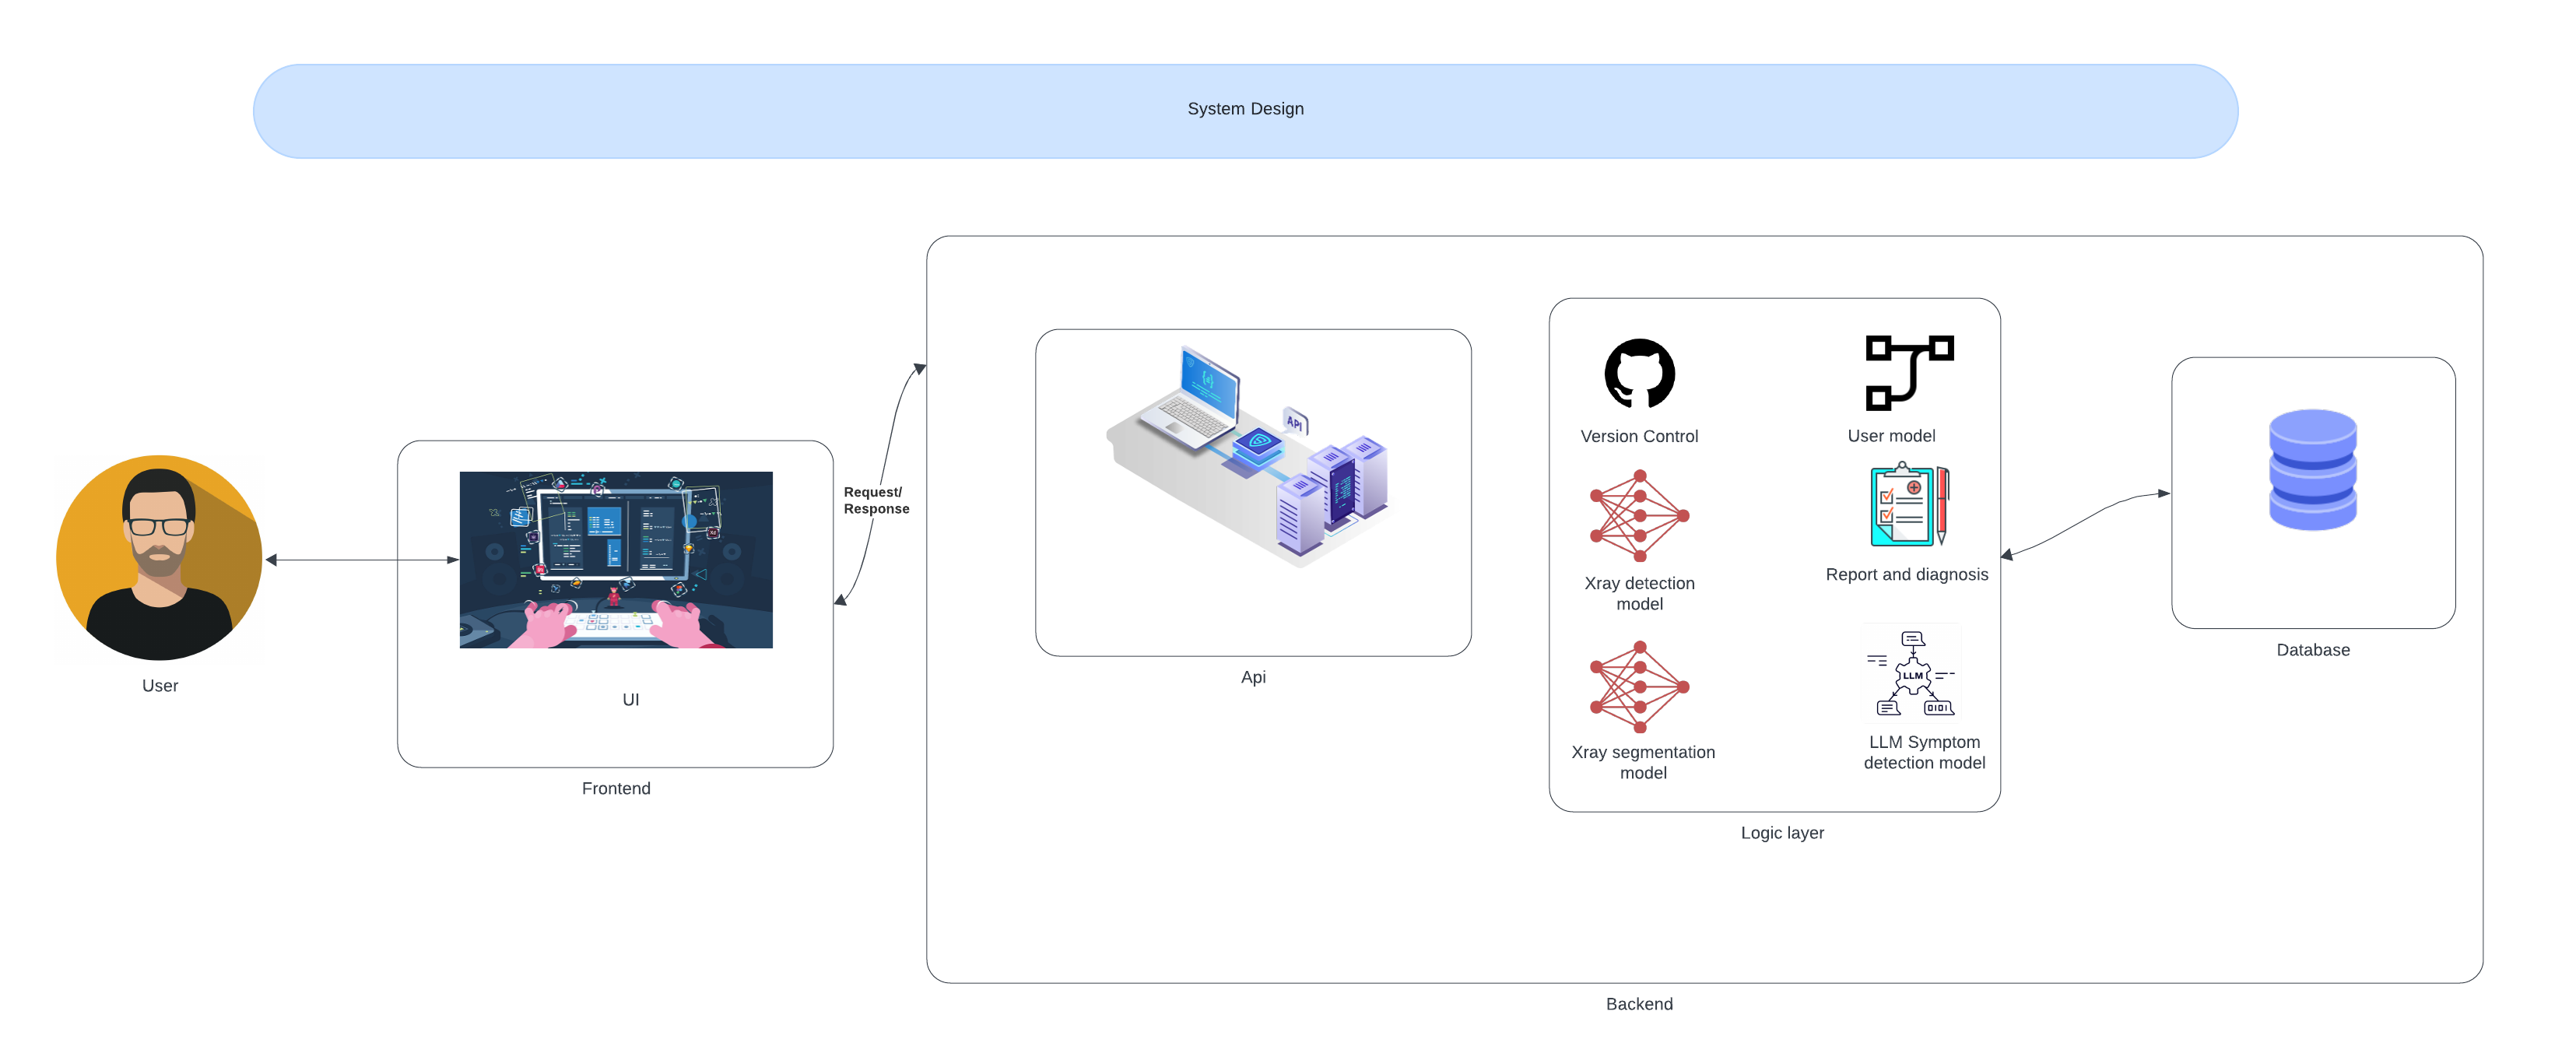
\includegraphics[width=0.8\textwidth]{Figures/System_design_diagram.png}
  \caption{Overall System Architecture.}
  \label{fig:architecture}
\end{figure}


\subsubsection{Frontend}
The frontend consists of a web interface and a mobile application. The web interface allows users to access the AI Assistant from a web browser, while the mobile application provides a convenient and portable platform for interacting with the system.

\subsubsection{Backend}
\begin{itemize}
    \item \textbf{Logic}
    \begin{itemize}
        
        \item \textbf{Symptom Analysis: } The business layer processes user-provided symptoms, analyzes them, and generates a list of potential medical conditions.
        \item \textbf{Diagnosis Prediction: } Based on the symptom analysis, the system predicts potential diagnoses and provides relevant medical advice.
        \item \textbf{Referral Generation: } If necessary, the system generates referrals to specialized healthcare providers based on the predicted diagnosis.

    \end{itemize}

    \item \textbf{API}
    \begin{itemize}
        \item \textbf{User Management: } Manages user authentication, profile information, and privacy settings.
        \item \textbf{Chatbot Interaction: } Handles user interactions with the chatbot, including symptom input, medical advice, and referral generation.
        \item \textbf{Image Analysis: } Processes uploaded medical images, performs analysis, and generates diagnostic reports.
    \end{itemize}

    \item \textbf{Data Layer}
    \begin{itemize}
        \item \textbf{User Data: } Stores user profiles, chat history, and feedback.
        \item \textbf{Medical Data: } Contains information about medical conditions, treatments, and referrals.
        \item \textbf{Image Data: } Stores uploaded medical images and diagnostic reports.
    \end{itemize}
\end{itemize}


\subsection{Data Design}

\subsubsection{Data Collection}


\begin{figure}[H]
    \centering
    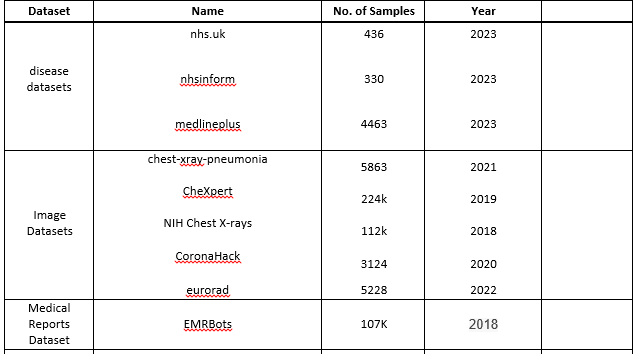
\includegraphics[width=0.6\textwidth]{./Figures/data.png}
    \caption{Data Collection Process.}
    \label{fig:datacollection}
\end{figure}

\textbf{Textual Data Collection}
The textual data for conditions and treatments was collected from the NHS (National Health Service) website, specifically from the section dedicated to medical conditions. This section provides comprehensive information about various health conditions, including their symptoms, causes, treatments, and other relevant details.

Efforts were made to systematically gather information from multiple pages within this section of the NHS website. This involved extracting structured data about different medical conditions, ensuring accuracy and consistency in the dataset.

By utilizing reputable sources such as the NHS website, we aim to ensure the reliability and credibility of the collected data, thereby enhancing the effectiveness and validity of the Machine Learning (ML) and Large Language Model (LLM) models trained on this dataset.


\textbf{Image Data Acquisition}
The chest X-ray images used in this study were obtained from two primary sources: the CheXpert dataset and the NIH Chest X-ray dataset (CXR14).

The CheXpert dataset is a large publicly available dataset consisting of chest radiographs and associated radiological reports. It contains a diverse range of chest X-ray images with annotations for various abnormalities, allowing for the training and evaluation of machine learning models.

The NIH Chest X-ray dataset (CXR14)  is another widely used dataset comprising chest X-ray images collected from the National Institutes of Health Clinical Center. It provides a substantial collection of chest X-ray images with associated labels, enabling researchers to develop and validate algorithms for various medical imaging tasks.

Images from both datasets were collected in various file formats and resolutions, reflecting the real-world variability encountered in medical imaging. Preprocessing techniques were applied to standardize the images and enhance their quality before further analysis.

\textbf{Textual Data Transformation}
To enhance the utility and accessibility of the textual data collected, a comprehensive transformation process was employed. This involved two main steps, each leveraging the collective capabilities of several Large Language Models (LLMs) to reduce model bias and improve the diversity of the data interpretations.

\begin{itemize}
    \item \textbf{Symptom Summarization}
    The first step in the transformation process was to distill complex medical descriptions from the collected datasets into concise bullet points. These summaries are crucial for quick reference within the Medibot system and for ensuring that users receive straightforward and digestible medical information. We utilized a blend of advanced LLMs, including GPT-4 and Llama3-70b, to achieve a balance of accuracy and clarity, minimizing bias by integrating multiple model insights.
    
    
    \item \textbf{Generation of Interactive Queries}
    Following the summarization, the next step was to create dynamic and interactive content that would facilitate a naturalistic interaction between users and Medibot. This involved generating potential questions that patients might ask based on their symptoms, as well as crafting statements that patients could use to describe their symptoms accurately to a doctor. For this task, a combination of LLMs including GPT-3.5, Llama3-70b, and the Mixture of Experts (MoE) model Mixtral22b*8 were used. This ensemble approach ensured that the generated questions and descriptions were varied, realistic, and free from the biases typically associated with single-model outputs.
    
\end{itemize}
By integrating multiple LLMs at each stage of the textual data transformation process, we mitigated the risks of model bias, ensuring that the outputs were nuanced and broadly applicable. This methodology supports Medibot's goal to provide reliable and user-friendly diagnostic interactions.

\textbf{Data Augmentation for Image Data}
To ensure that our AI models are robust and capable of handling real-world variability in medical imaging, we applied a comprehensive data augmentation strategy to our image dataset. This approach involved simulating a variety of conditions that images might undergo in practical settings, particularly those captured using mobile devices.

\begin{itemize}
    \item 
    \textbf{Augmentation Techniques Implemented}
    We employed a diverse set of image transformations to mimic various photographic effects and artifacts. These included:
    \begin{itemize}
        \item \textbf{Moire Patterns} to simulate the interference effects seen in digital images.
        \item \textbf{Blur} to replicate out-of-focus images.
        \item \textbf{Motion Blur} to mimic the effect of camera movement during exposure.
        \item \textbf{Glare} (both matte and glossy) to represent light reflections on different surfaces.
        \item \textbf{Tilt} for angular misalignments.
        \item \textbf{Brightness Adjustments} (both increases and decreases).
        \item \textbf{Contrast Adjustments} (both increases and decreases).
        \item \textbf{Rotation and Translation} to simulate changes in camera orientation and position.
        \item \textbf{Exposure Variation} to mimic under and over-exposed images.
    \end{itemize} 

    \item \textbf{Application of Augmentations}
    To integrate these augmentations effectively, we randomly applied between one to five of these filters to 70\% of the images in our dataset. This method allowed us to create a range of scenarios, from minor alterations to more severely altered images, thereby preparing our models to perform reliably under various photographic conditions.
    
    \item 
    \textbf{Objective and Benefits}
    The objective of implementing these diverse augmentation techniques was to train our AI models to recognize and interpret medical images accurately, regardless of the quality or source of the image. This is particularly crucial for images taken from mobile devices in less controlled environments. As a result, our models demonstrate enhanced adaptability and reduced susceptibility to overfitting, ensuring reliable diagnoses even from sub-optimal image inputs.
\end{itemize}



\subsection{Interaction Design}

\subsubsection{User Interaction}
Users interact with the system through a user-friendly interface, providing symptoms and receiving medical advice and referrals. Design choices for user interactions focus on simplicity, clarity, and responsiveness.

\begin{figure}[H]
    \centering
    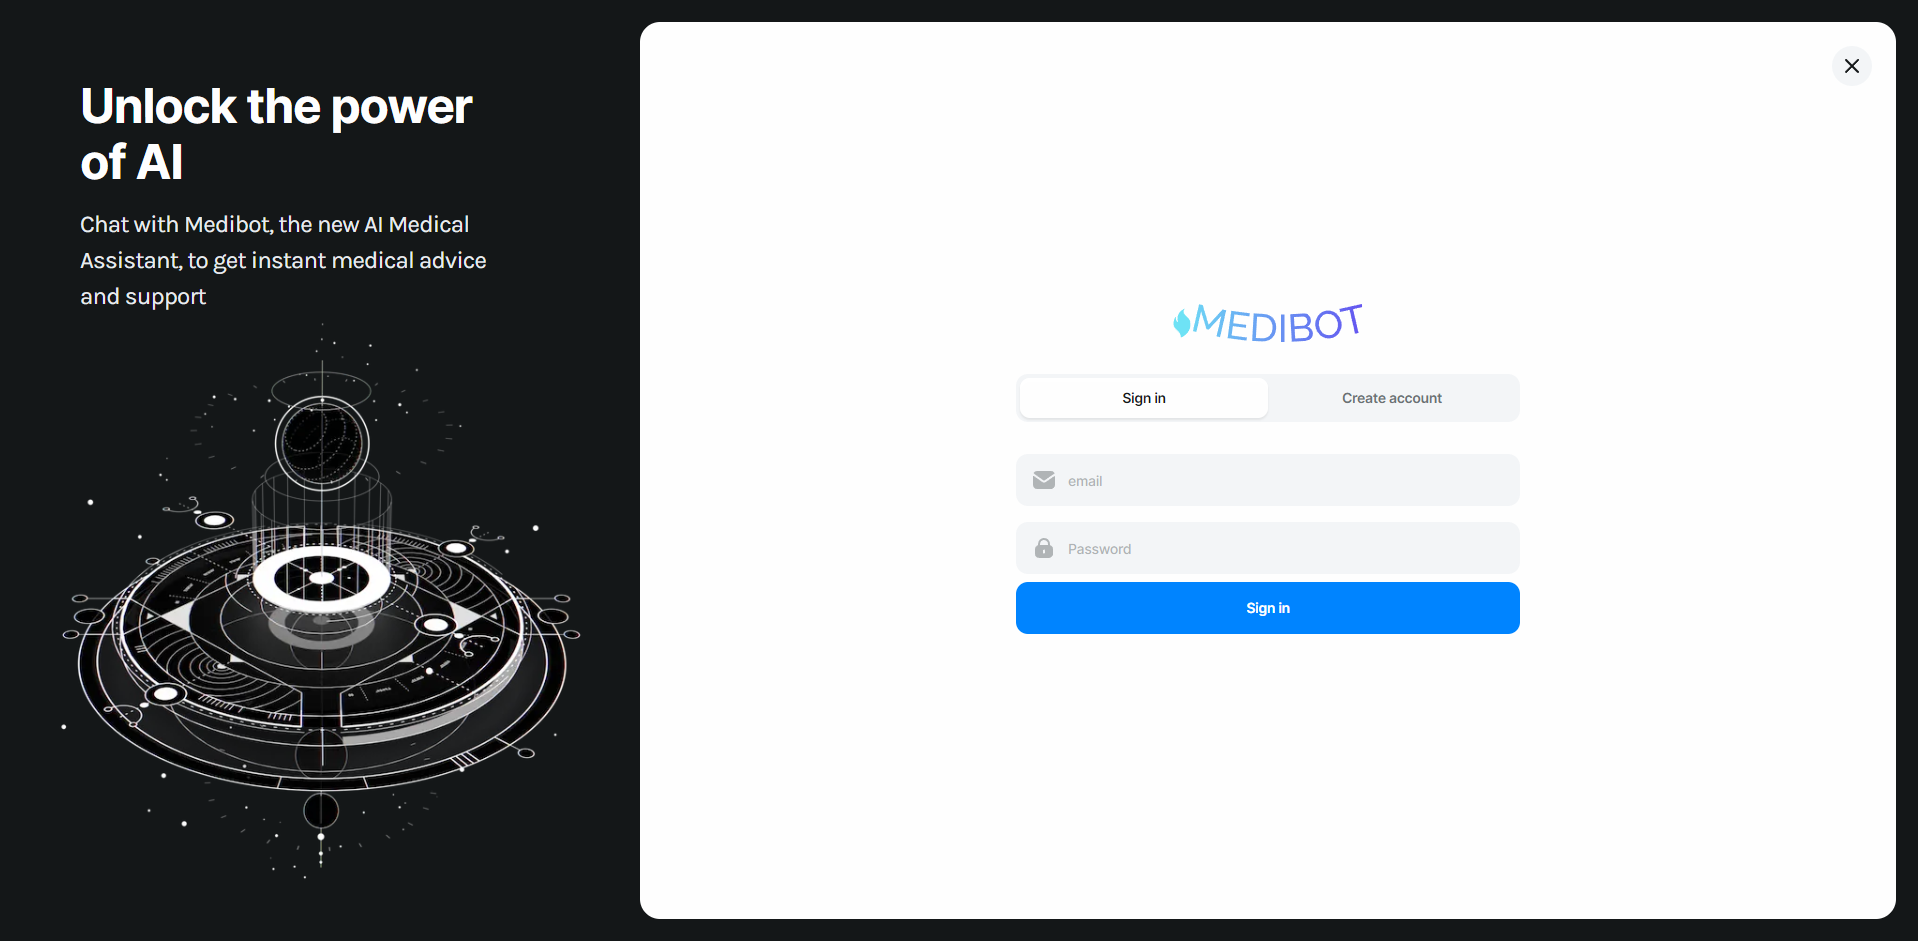
\includegraphics[width=0.6\textwidth]{./Figures/web-login.png}
    \caption{Web Login Page.}
    \label{fig:web-login}
\end{figure}
  
\begin{figure}[H]
    \centering
    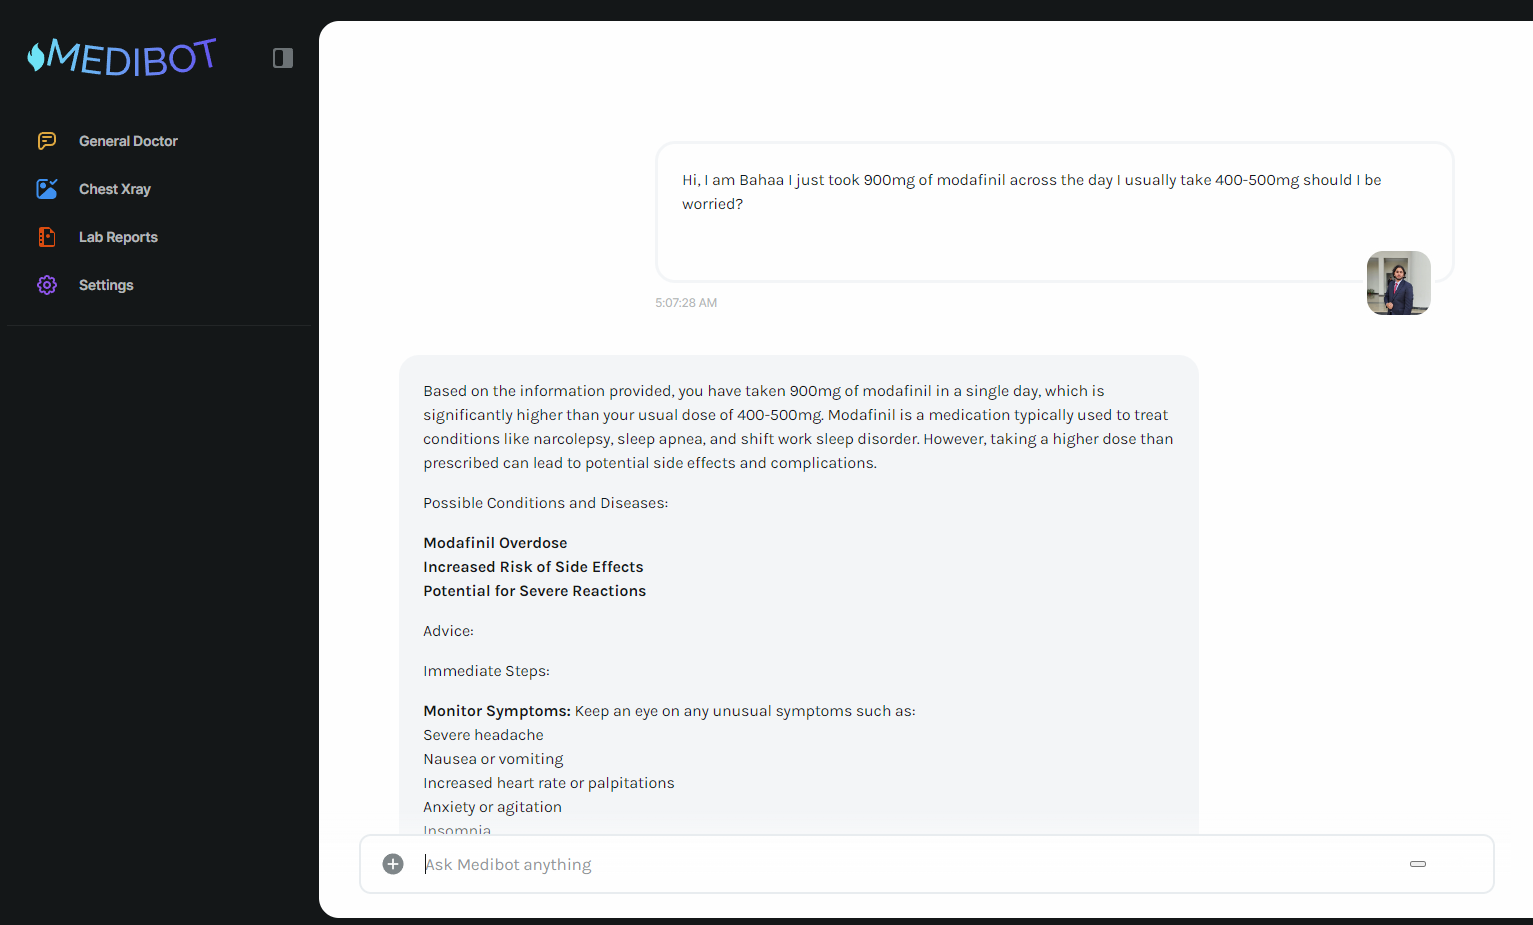
\includegraphics[width=0.6\textwidth]{./Figures/web-chat.png}
    \caption{Web Chat Page.}
    \label{fig:web-chat}
\end{figure}

\begin{figure}[H]
    \centering
    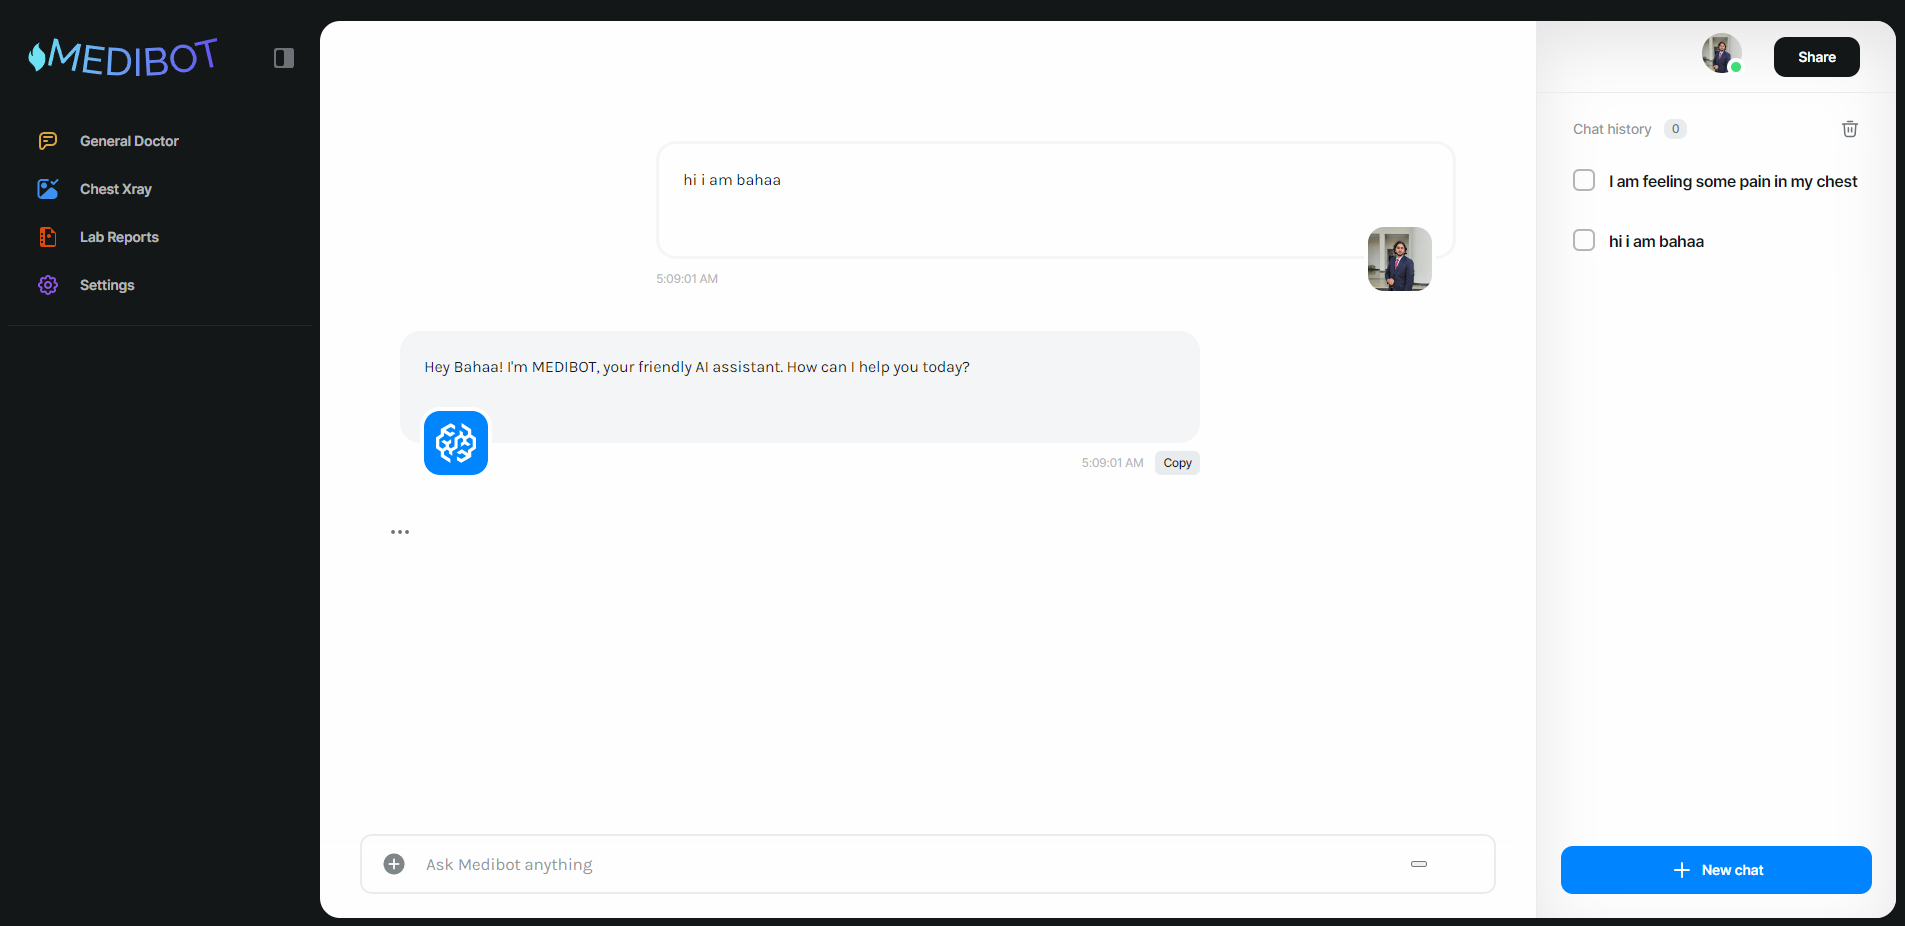
\includegraphics[width=0.6\textwidth]{./Figures/web-chat-history.png}
    \caption{Web Chat History Page.}
    \label{fig:web-chat-history}
\end{figure}

\begin{figure}[H]
    \centering
    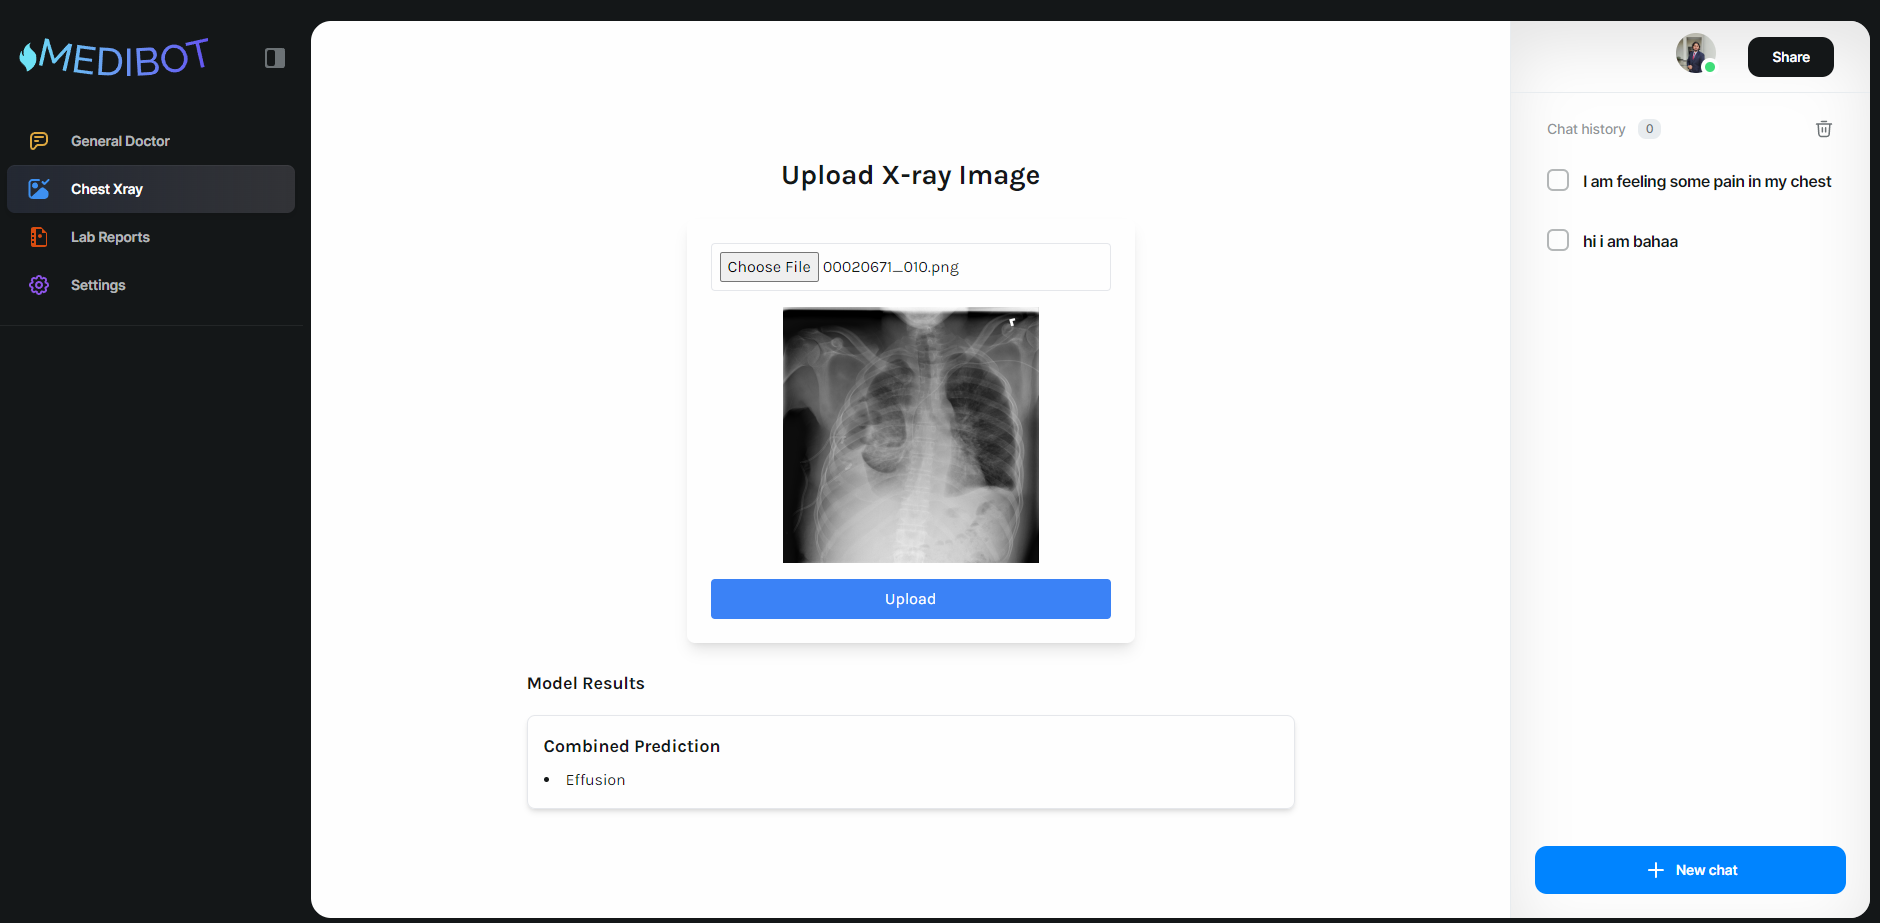
\includegraphics[width=0.6\textwidth]{./Figures/web-xray.png}
    \caption{Web Xray Diagnosis Page.}
    \label{fig:web-xray}
\end{figure}

\begin{figure}[H]
    \centering
    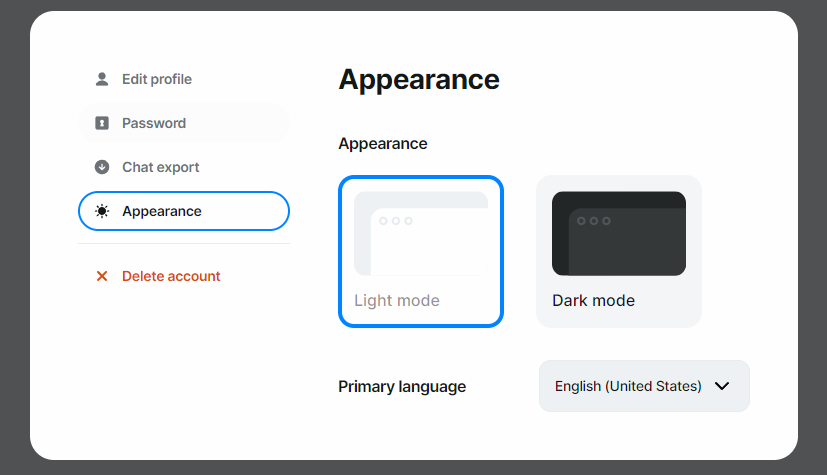
\includegraphics[width=0.6\textwidth]{./Figures/web-settings.png}
    \caption{Web Settings Page.}
    \label{fig:web-settings}
\end{figure}

\begin{figure}[htbp]
    \centering
    \begin{minipage}{0.3\textwidth}
        \centering
        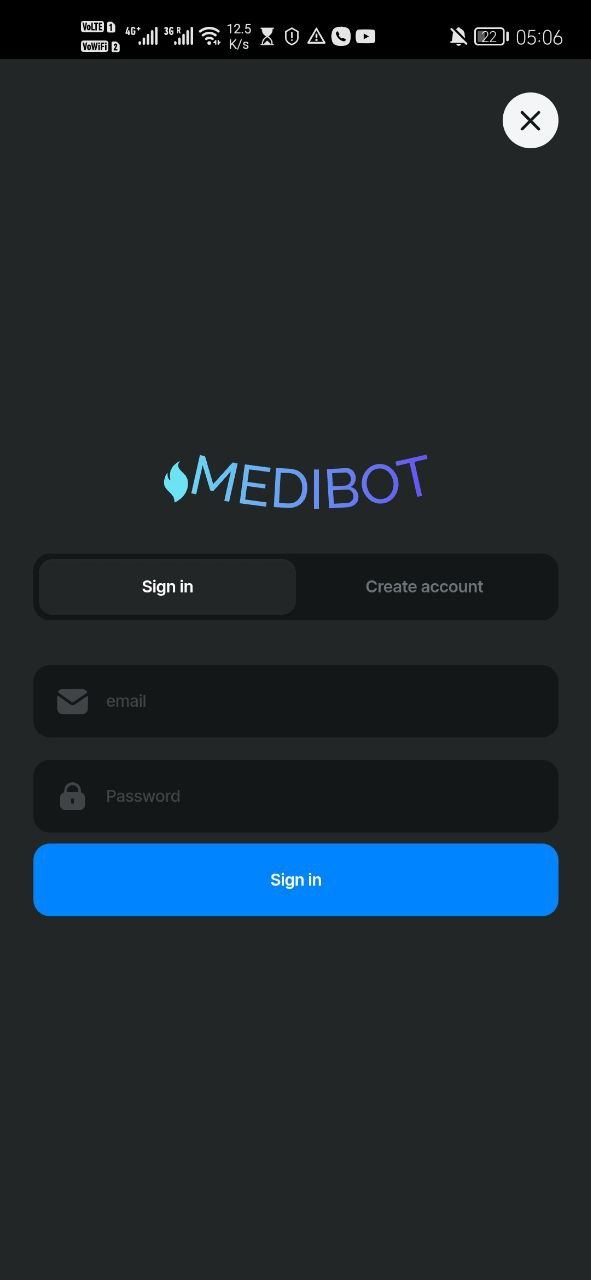
\includegraphics[width=\textwidth]{./Figures/mobile-login.jpg}
        \caption{Mobile Login Page}
        \label{fig:mobile-login}
    \end{minipage}\hfill
    \begin{minipage}{0.3\textwidth}
        \centering
        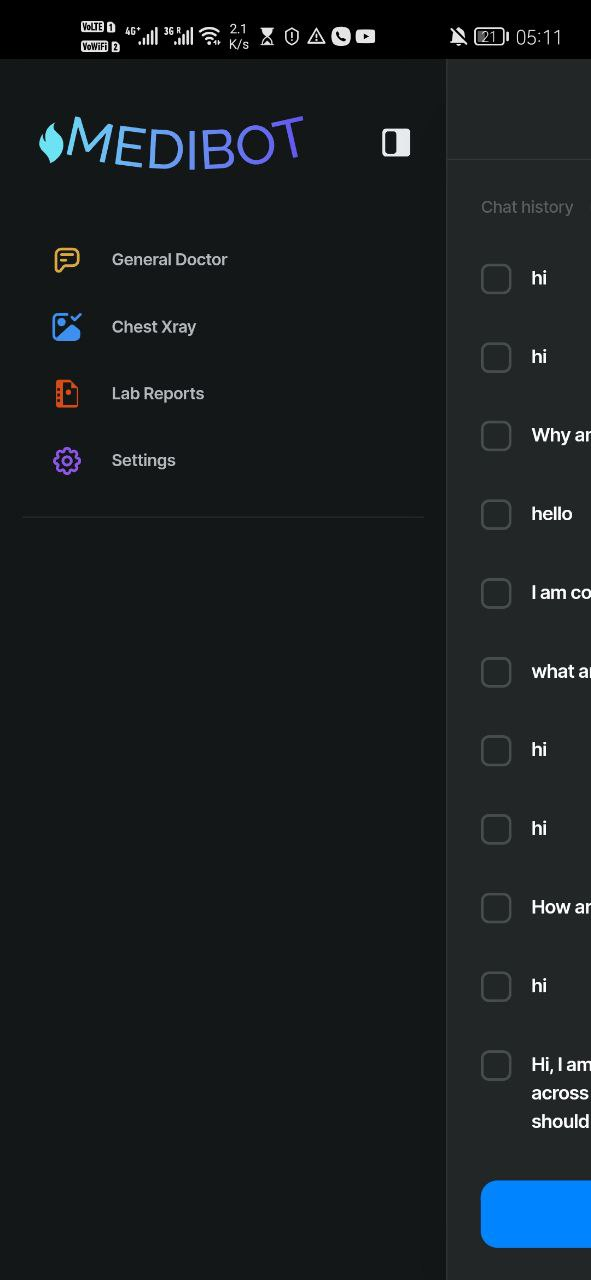
\includegraphics[width=\textwidth]{./Figures/mobile-menu.jpg}
        \caption{Mobile Menu Page}
        \label{fig:mobile-menu}
    \end{minipage}\hfill
    \begin{minipage}{0.3\textwidth}
        \centering
        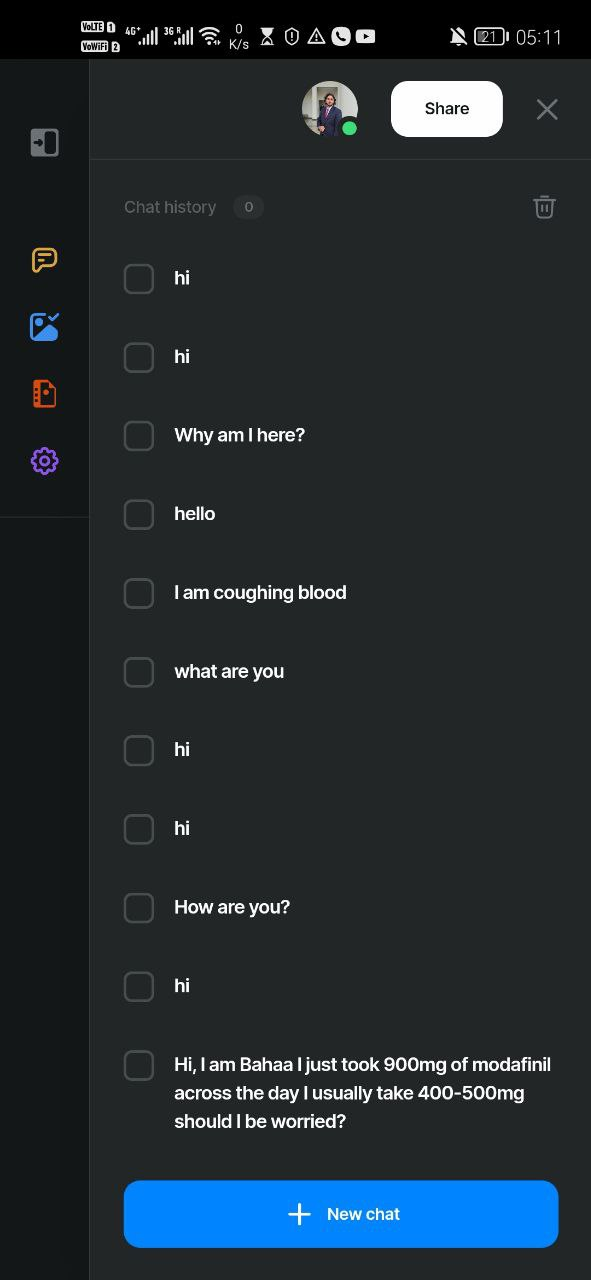
\includegraphics[width=\textwidth]{./Figures/mobile-chat-history.jpg}
        \caption{Mobile Chat History Page}
        \label{fig:mobile-chat-history}
    \end{minipage}
\end{figure}


\begin{figure}[htbp]
    \centering
    \begin{minipage}{0.3\textwidth}
        \centering
        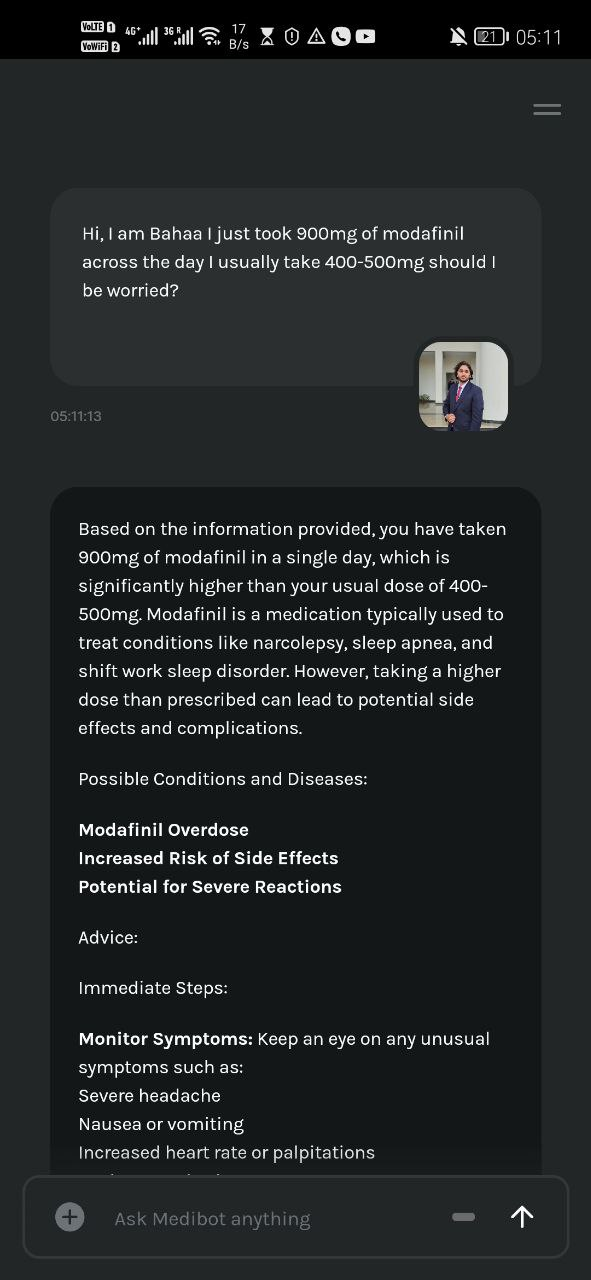
\includegraphics[width=\textwidth]{./Figures/mobile-chat.jpg}
        \caption{Mobile Chat Page}
        \label{fig:mobile-chat}
    \end{minipage}\hfill
    \begin{minipage}{0.3\textwidth}
        \centering
        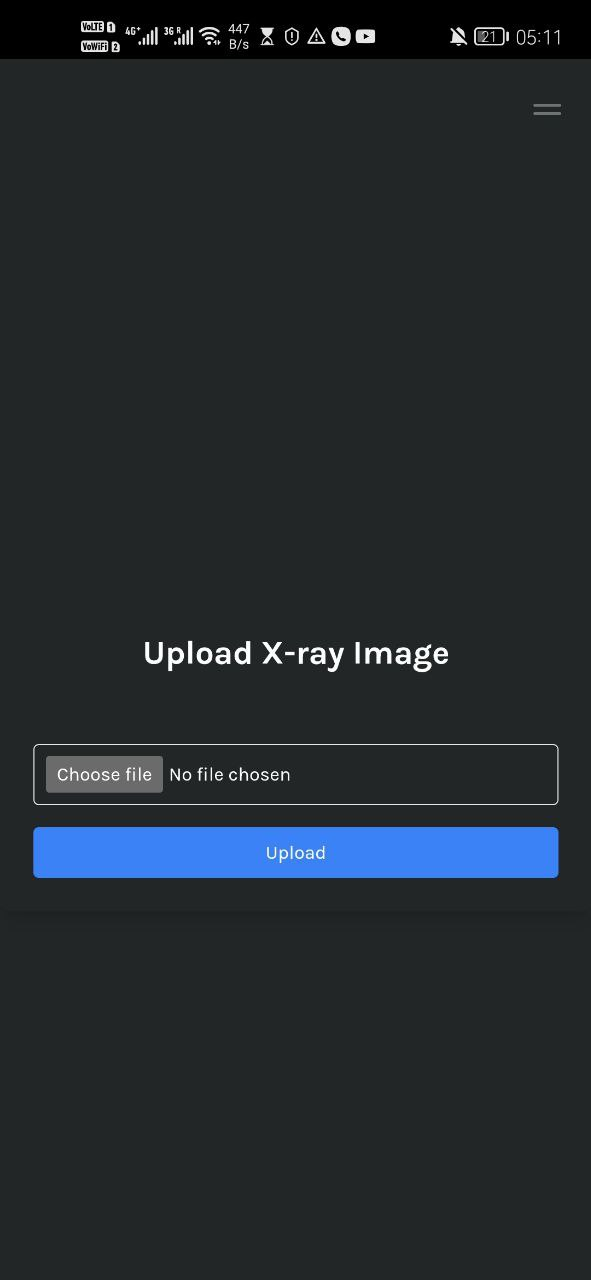
\includegraphics[width=\textwidth]{./Figures/mobile-xray.jpg}
        \caption{Mobile Xray Page}
        \label{fig:mobile-xray}
    \end{minipage}
\end{figure}

\clearpage



\subsection{Data Flow Diagrams}

\begin{figure}[H]
    \centering
    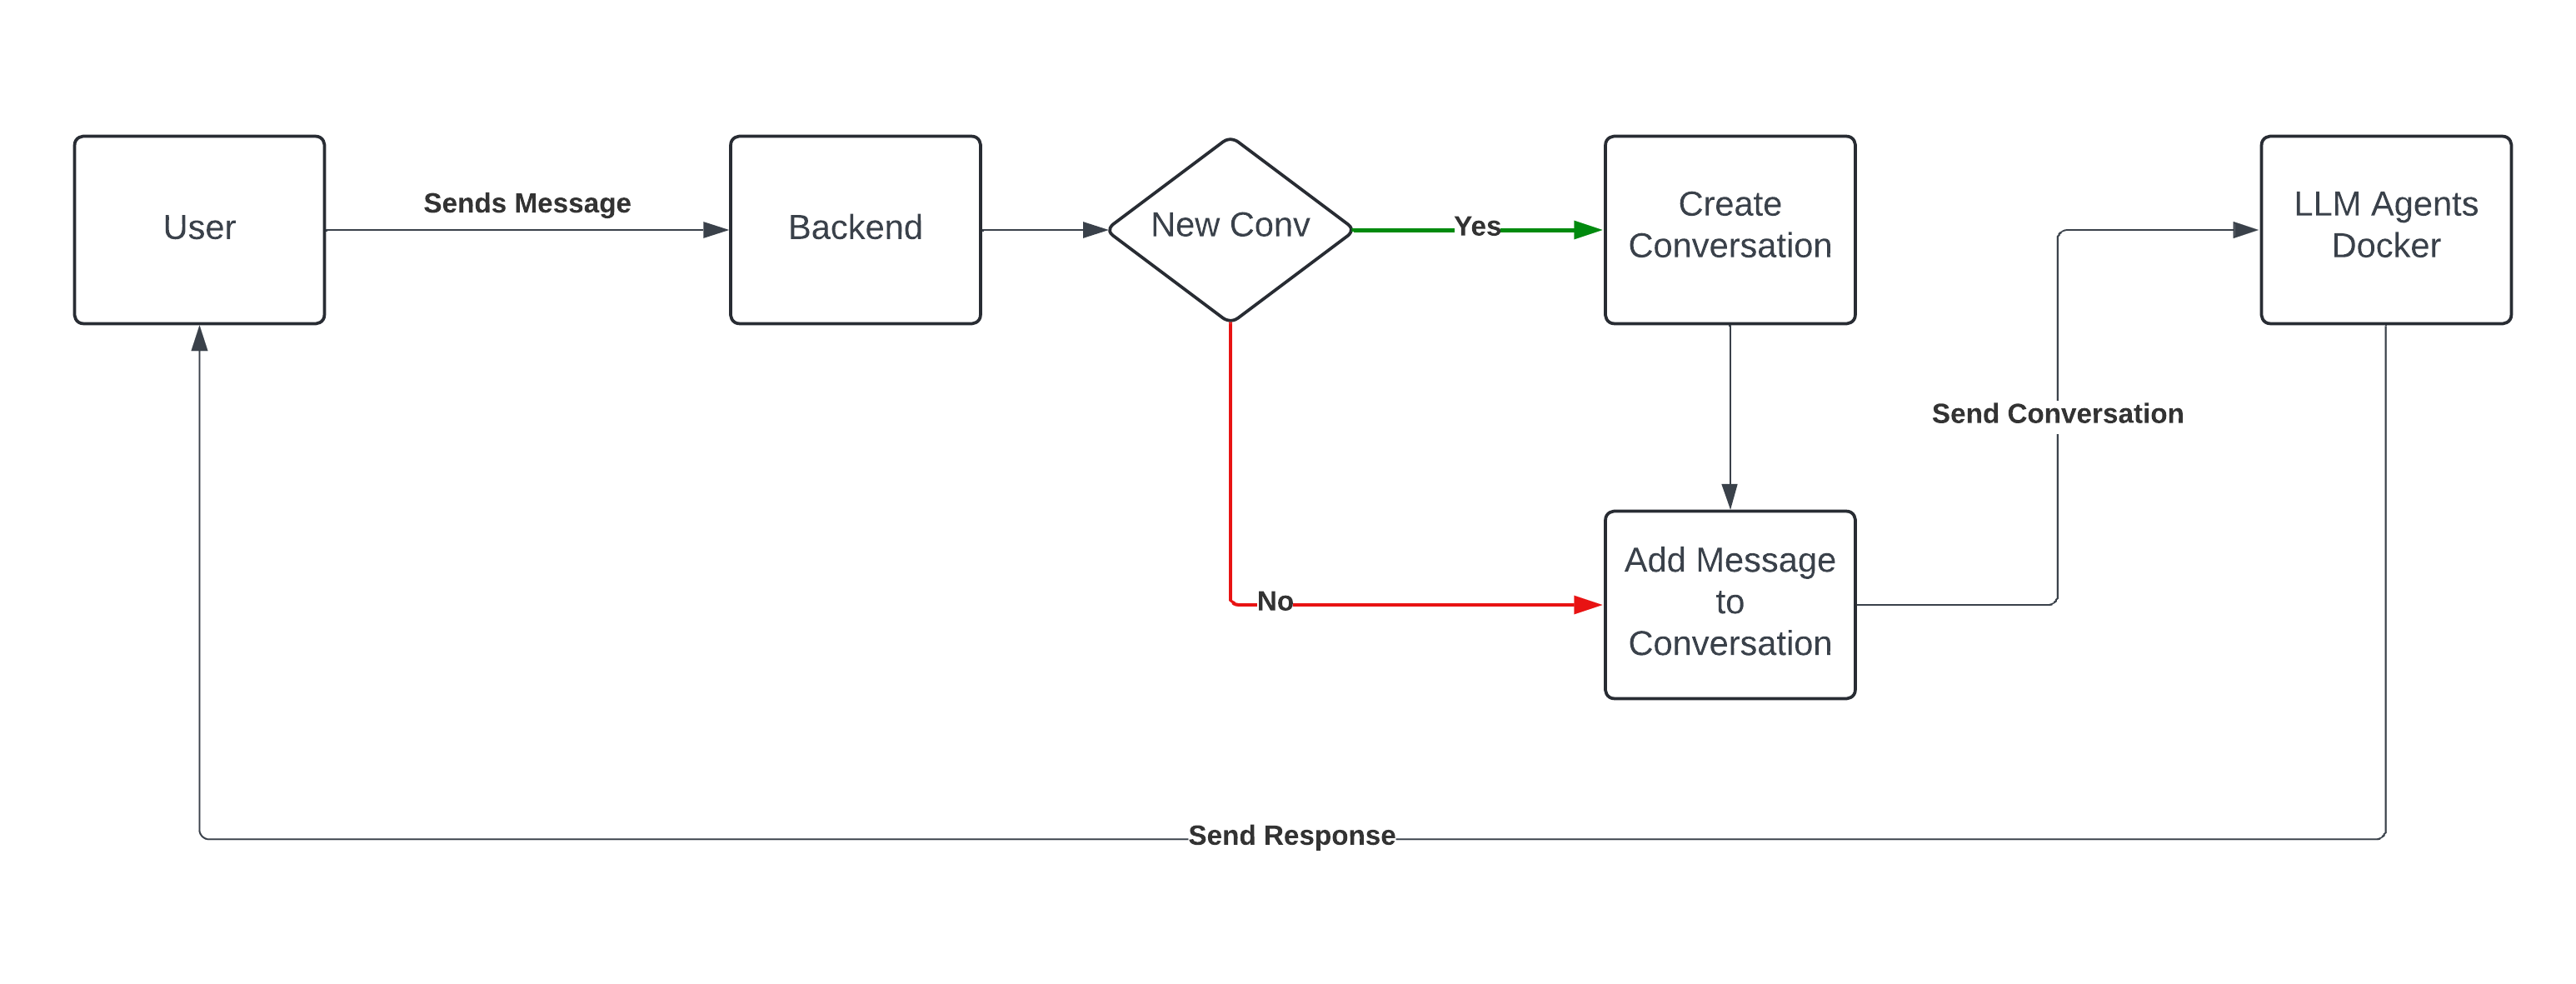
\includegraphics[width=0.6\textwidth]{./Figures/Dataflow Chat.png}
    \caption{Data Flow for Chat.}
    \label{fig:dataflow-chat}
\end{figure}

\begin{figure}[H]
    \centering
    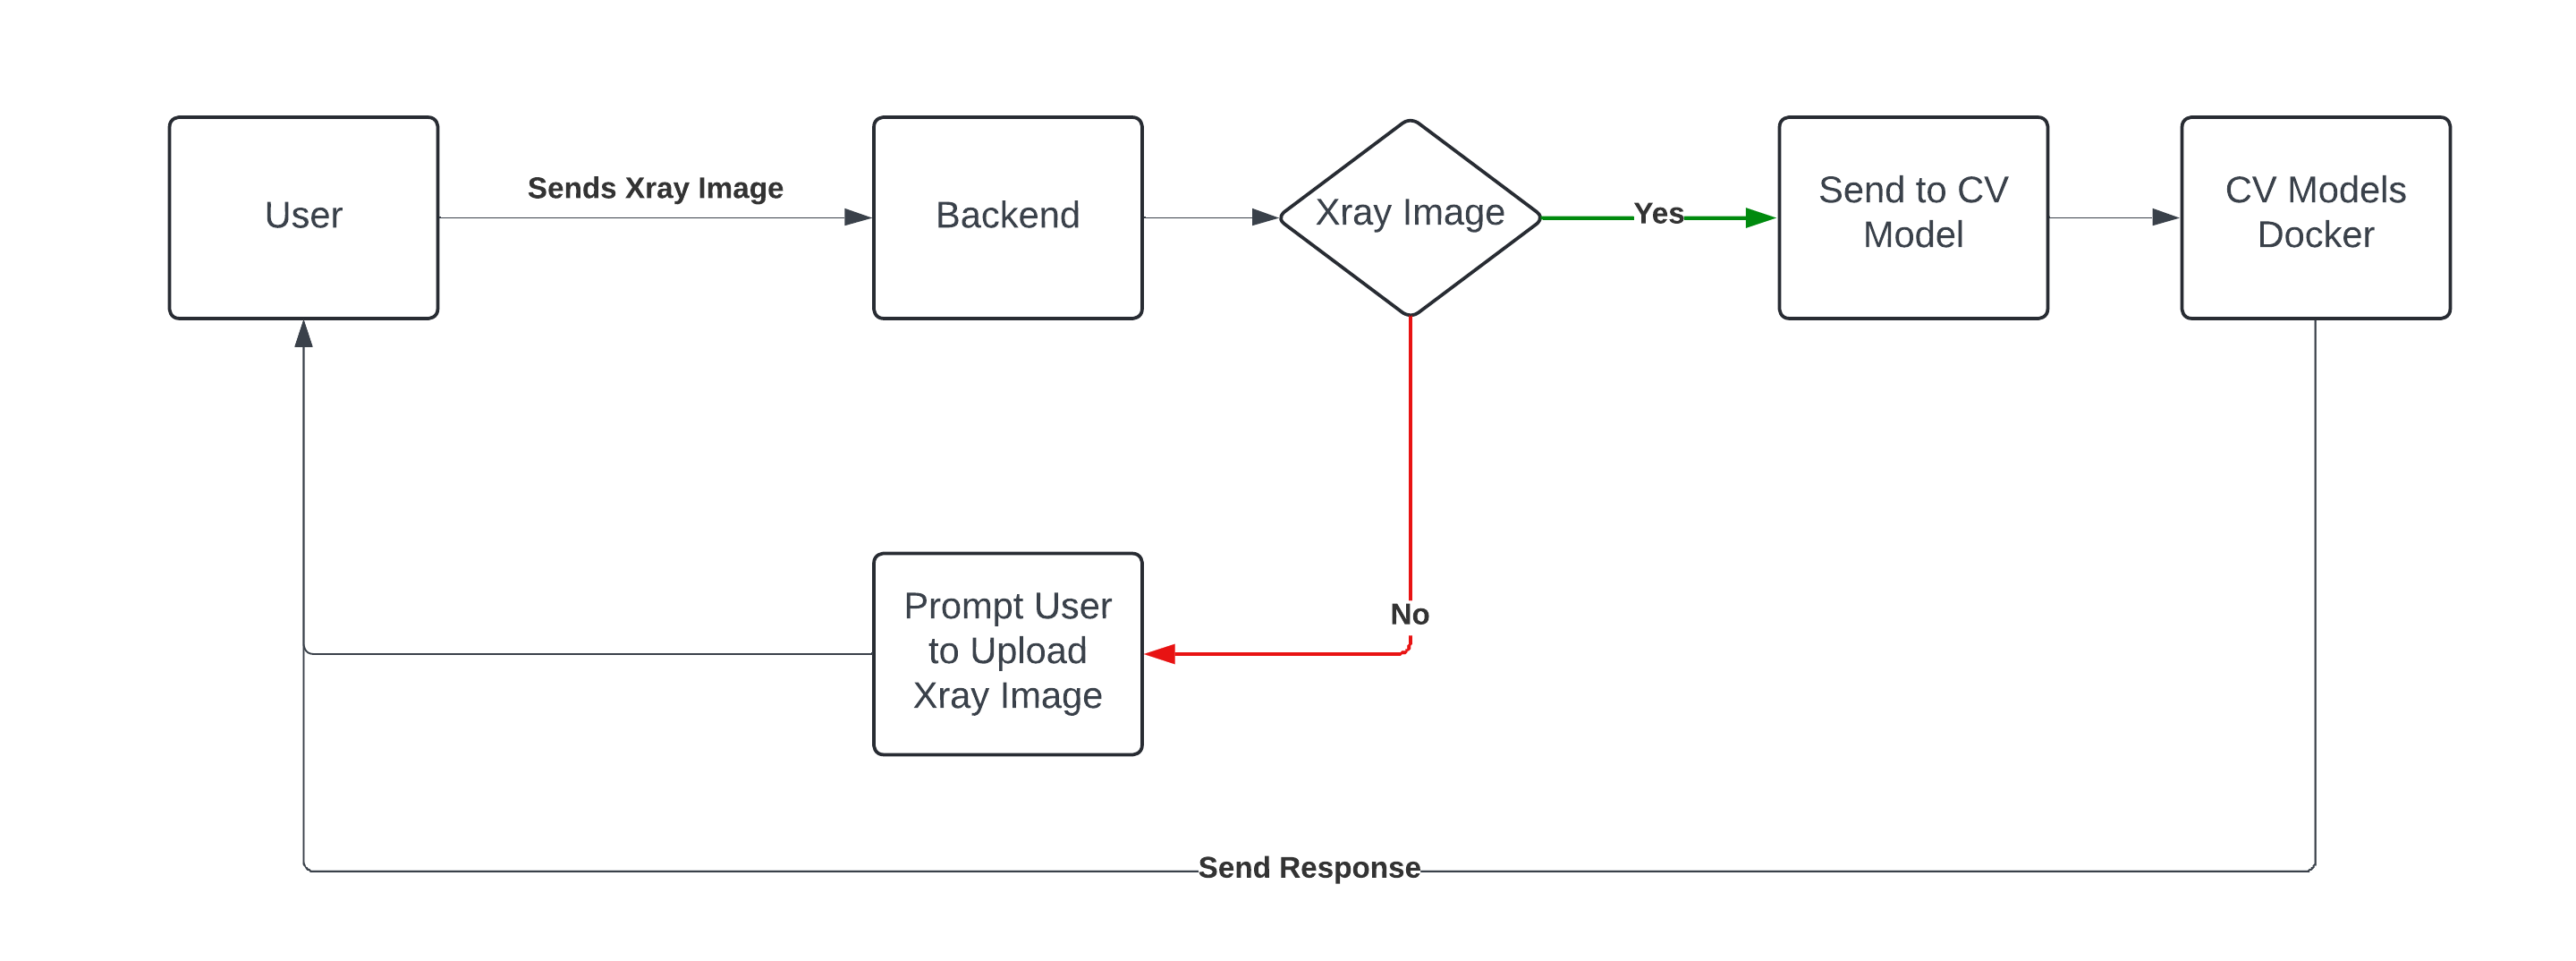
\includegraphics[width=0.6\textwidth]{./Figures/Dataflow Xray.png}
    \caption{Data Flow for Xray Analysis.}
    \label{fig:dataflow-xray}
\end{figure}

\begin{figure}[H]
    \centering
    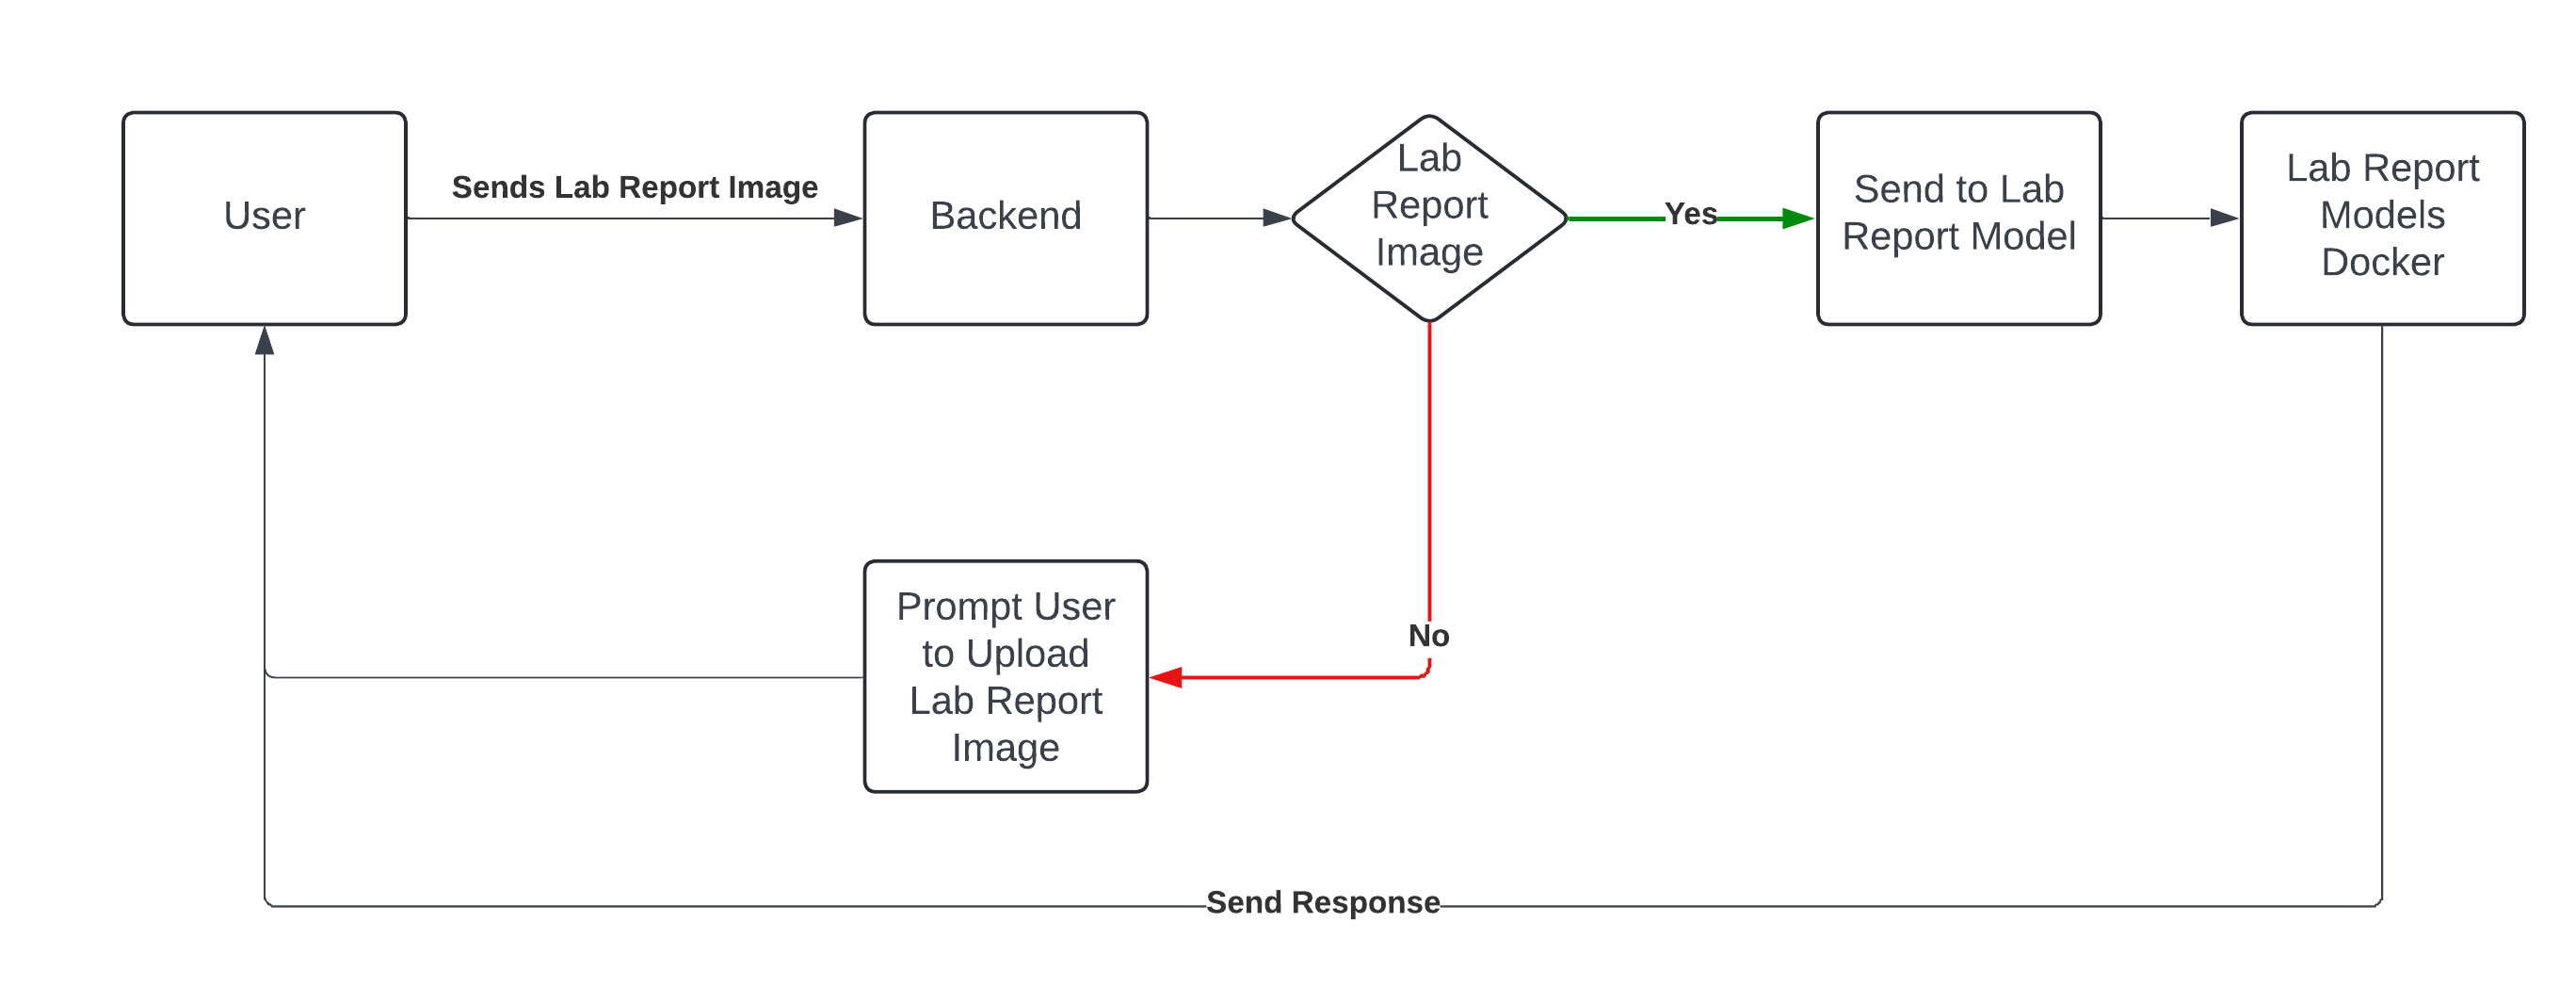
\includegraphics[width=0.6\textwidth]{./Figures/Dataflow Lab Report.png}
    \caption{Data Flow for Lab Report Analysis.}
    \label{fig:dataflow-lab-report}
\end{figure}

\begin{figure}[H]
    \centering
    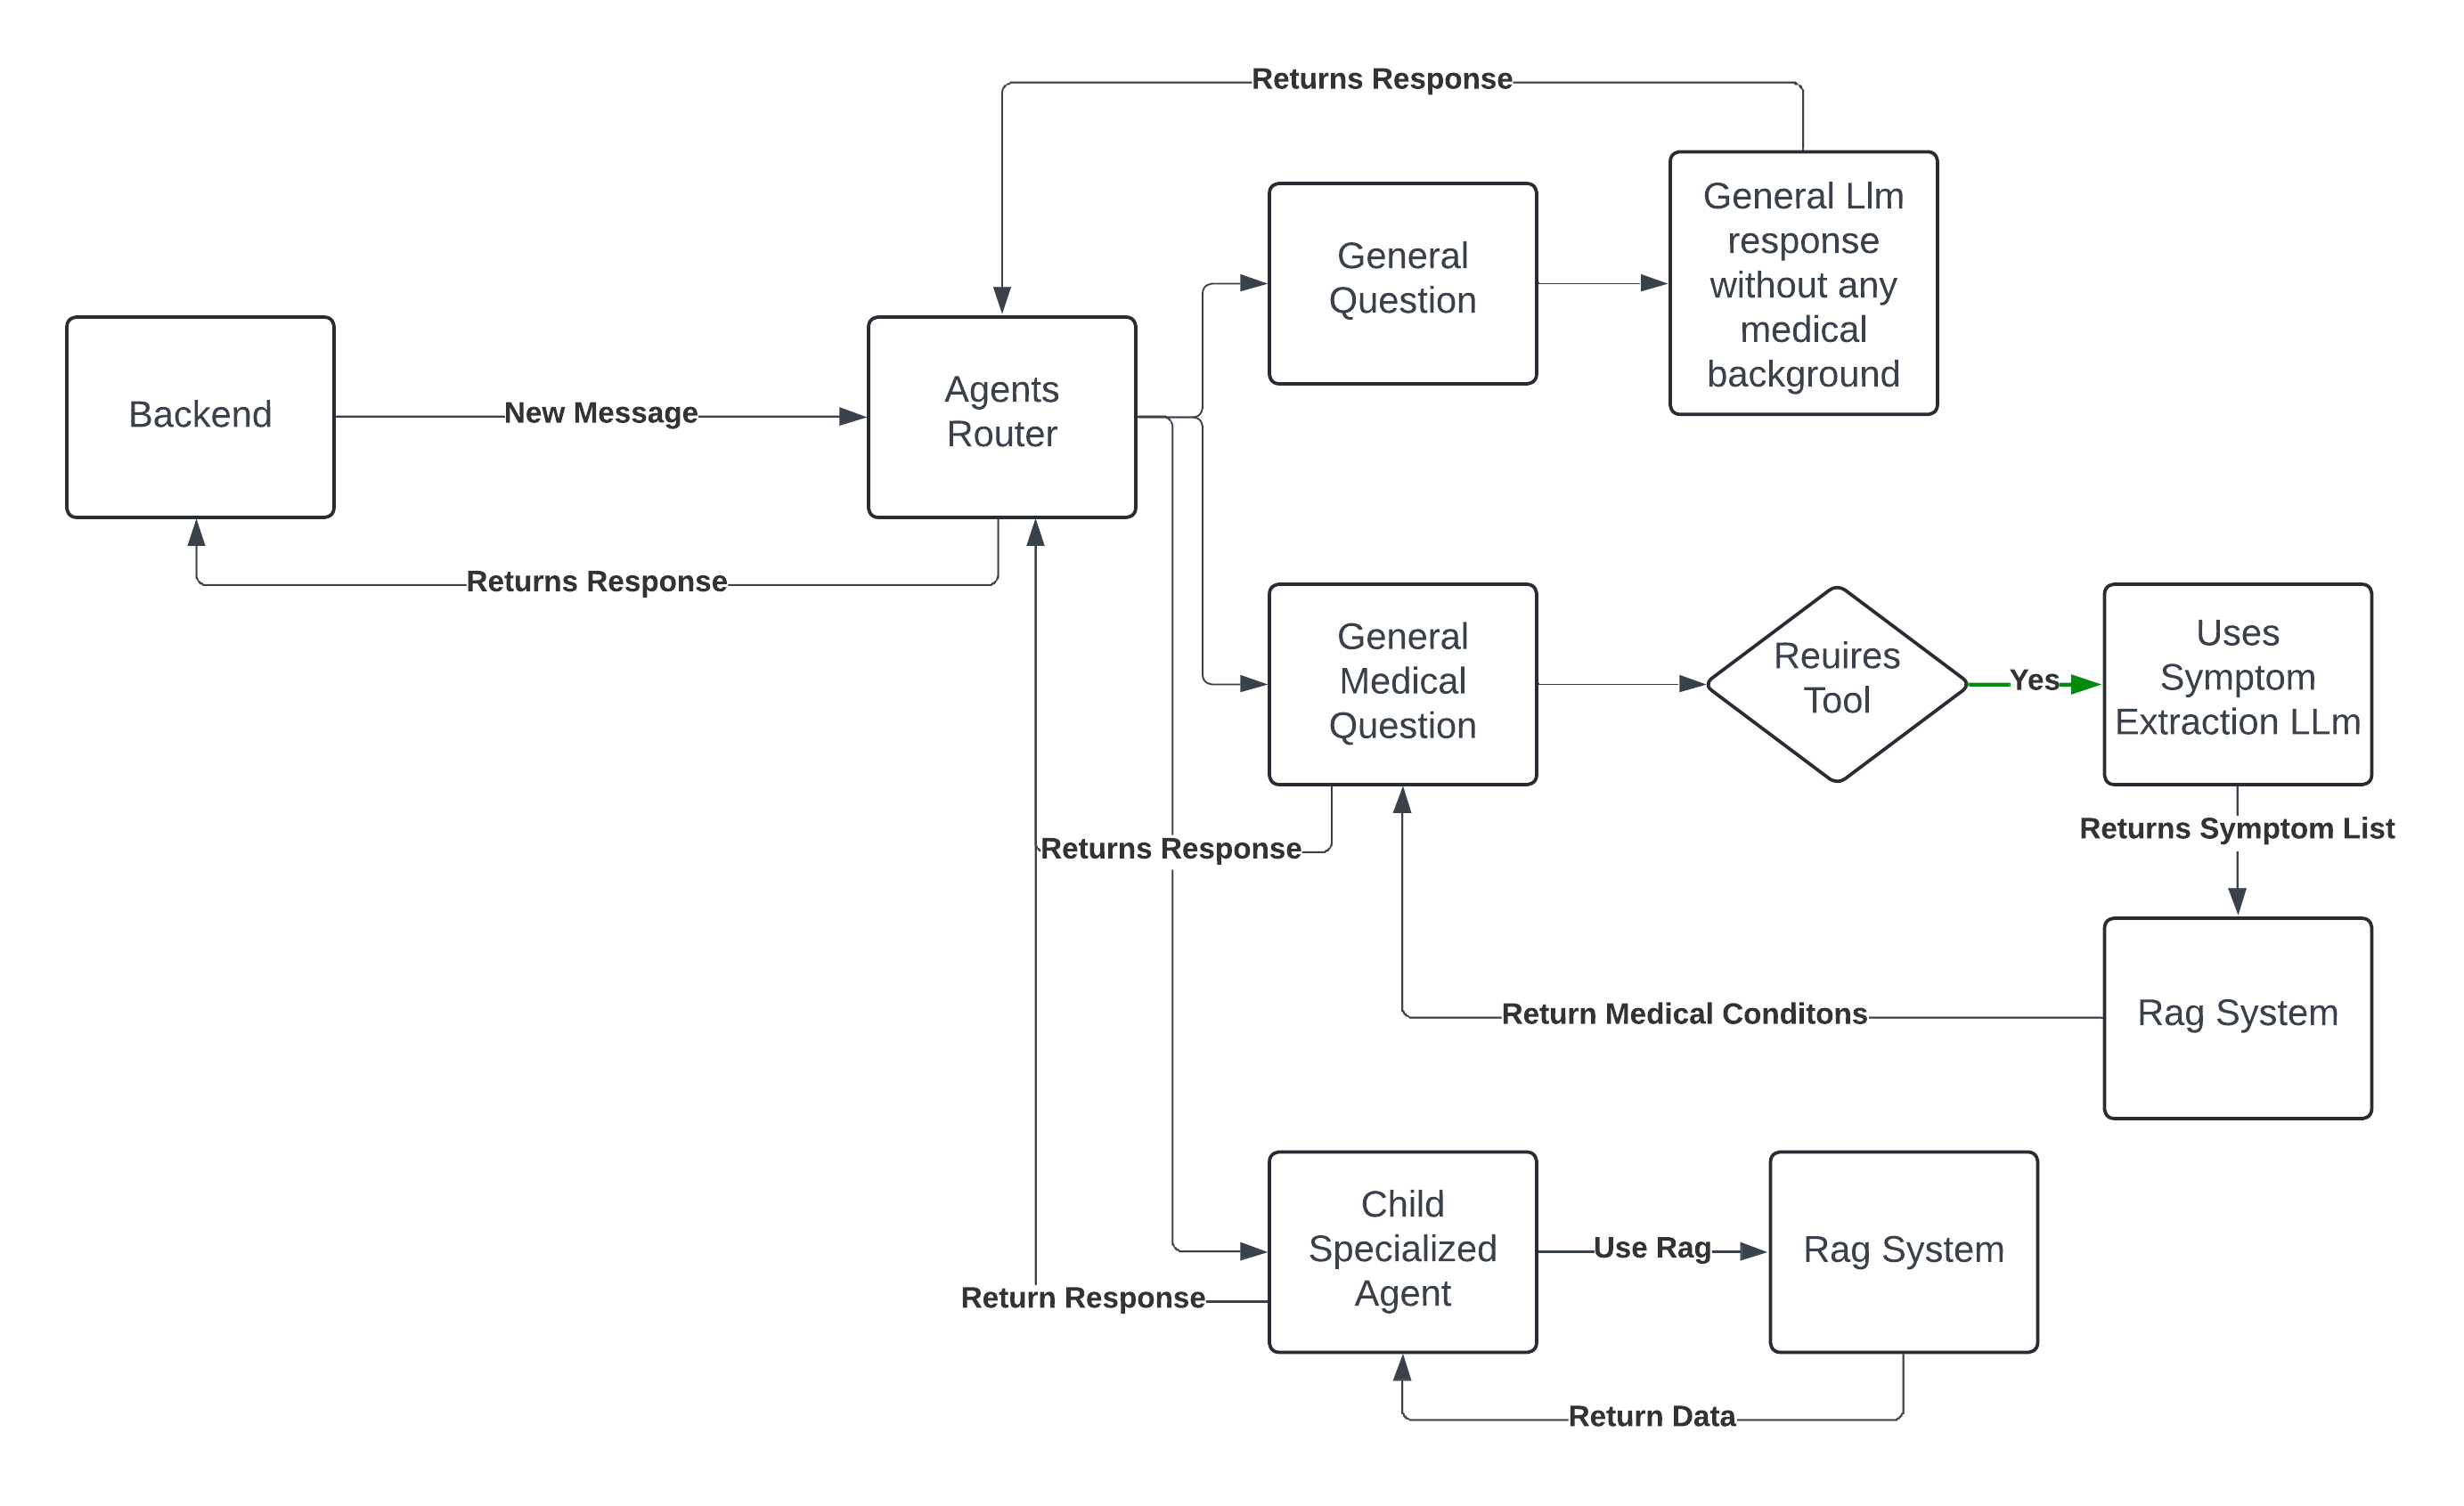
\includegraphics[width=0.6\textwidth]{./Figures/Dataflow Agents System.png}
    \caption{Data Flow for LLM Agents System.}
    \label{fig:dataflow-agents-system}
\end{figure}

\begin{figure}[H]
    \centering
    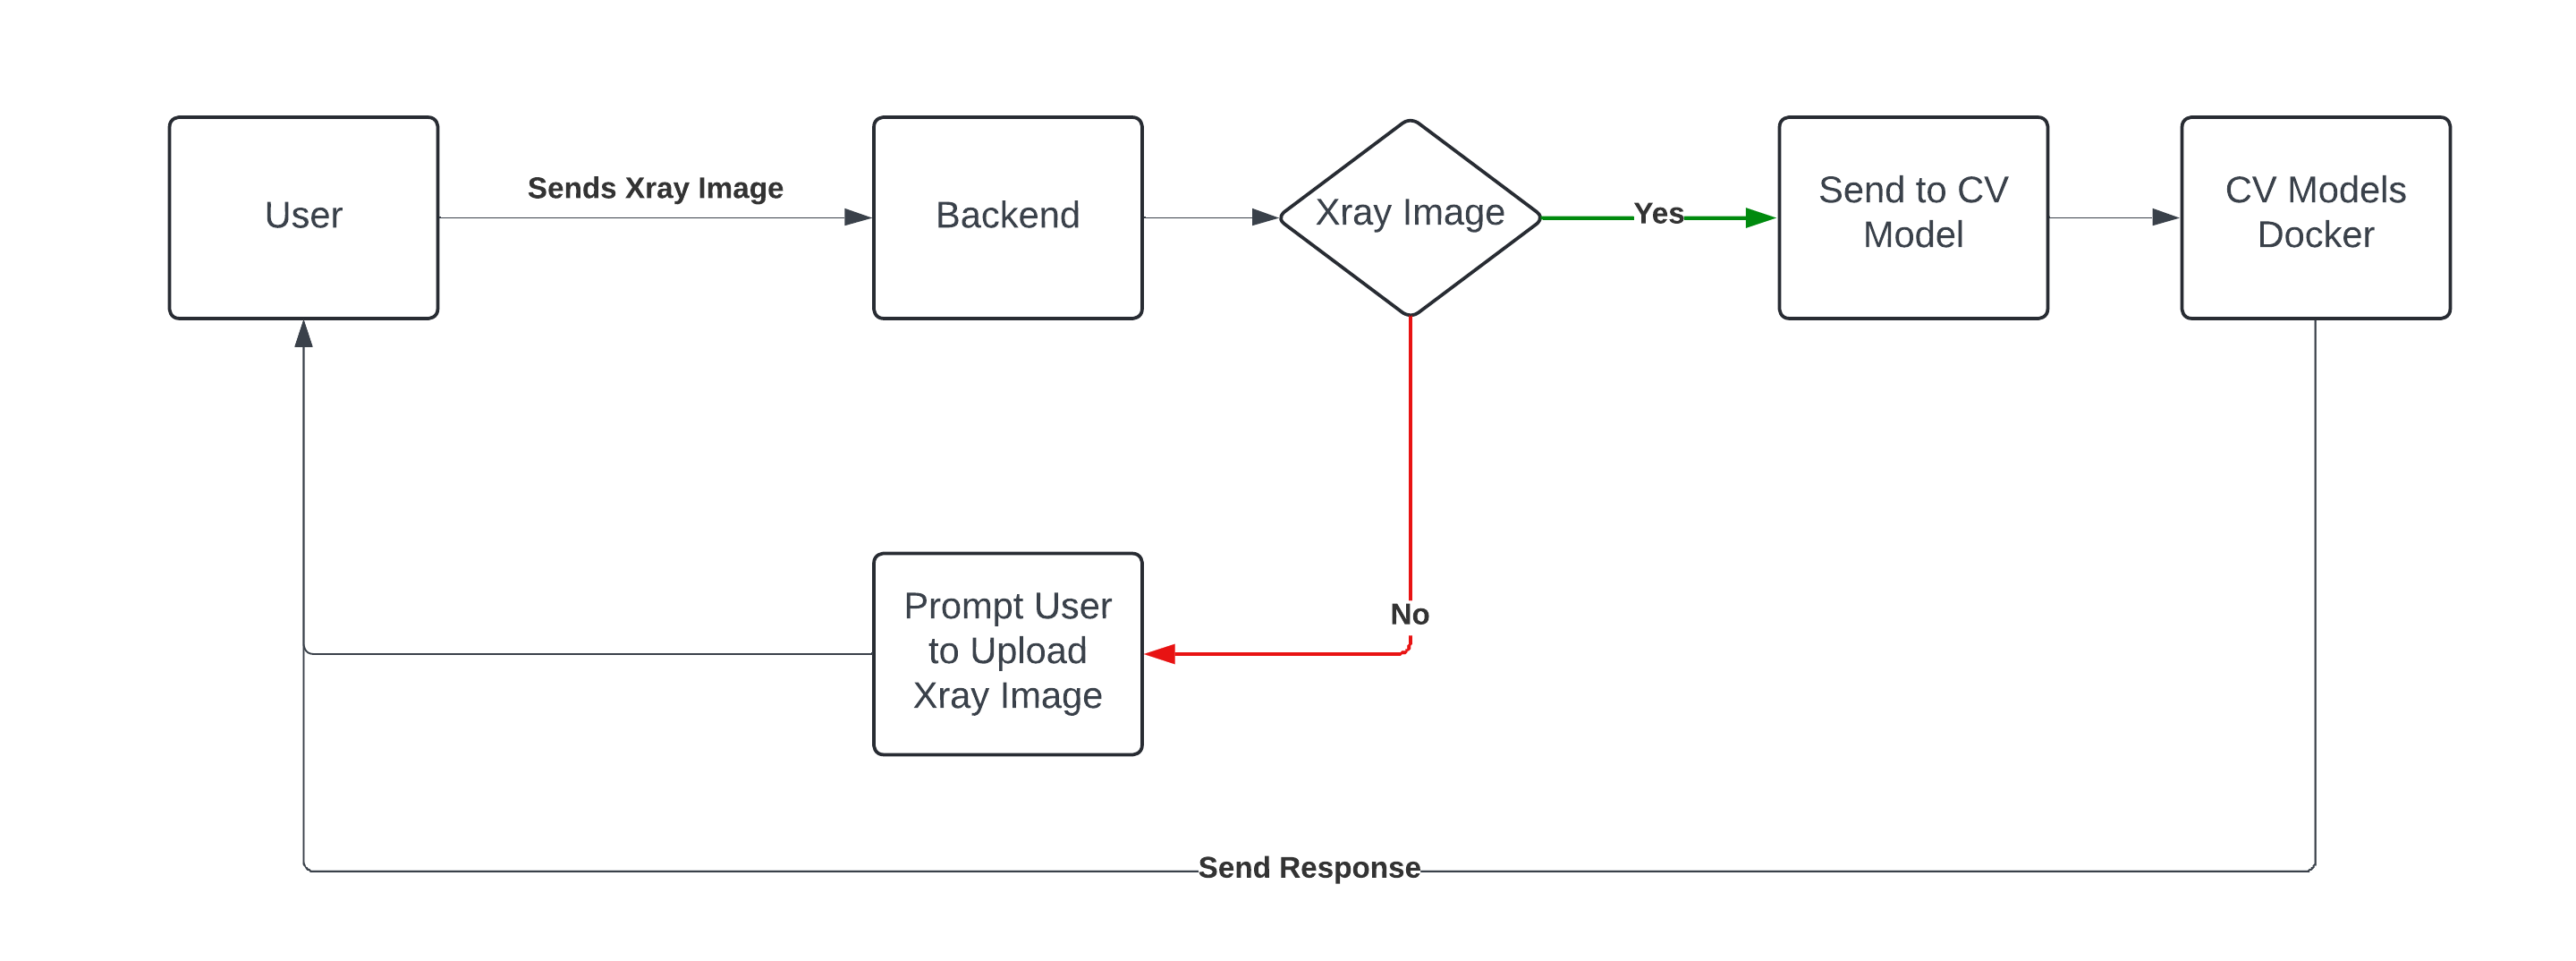
\includegraphics[width=0.6\textwidth]{./Figures/Dataflow Xray.png}
    \caption{Data Flow for Xray System.}
    \label{fig:dataflow-xray-system}
\end{figure}

\begin{figure}[H]
    \centering
    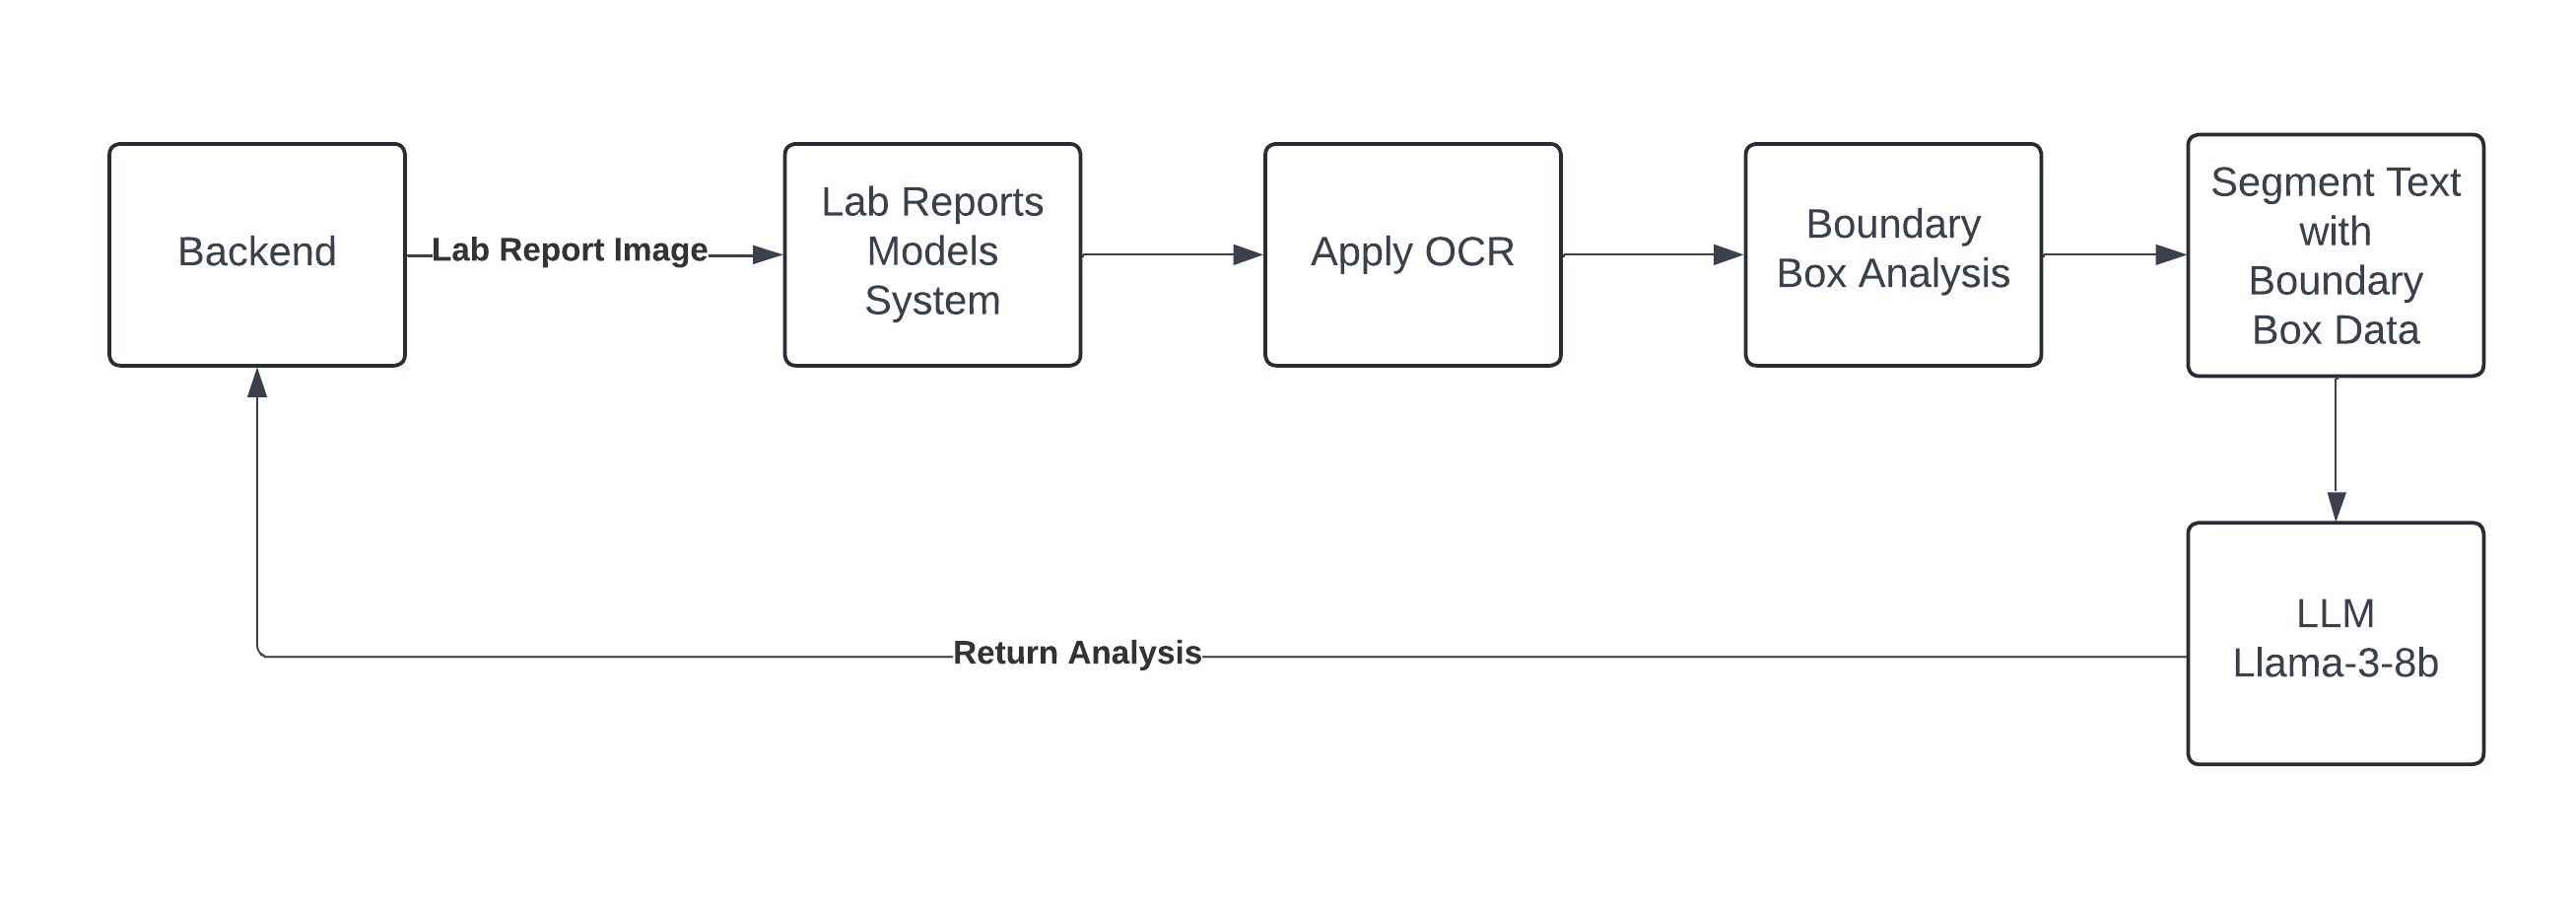
\includegraphics[width=0.6\textwidth]{./Figures/Dataflow Lab Reports.png}
    \caption{Data Flow for Lab Reports System.}
    \label{fig:dataflow-lab-reports-system}
\end{figure}


\subsection{Tools and Technologies}

\subsubsection{Software Frameworks}
The development of Medibot utilized several popular software frameworks and libraries, including:

\begin{itemize}
    \item \textbf{Python and FastAPI:} Employed throughout the backend development for its robust libraries and simplicity. FastAPI was specifically chosen for building high-performance APIs for the LLM agents, offering easy asynchronous support and scalability.

    \item \textbf{Node.js:} Served as the runtime environment for the entire system's backend, enabling asynchronous event-driven programming that supports non-blocking I/O operations. This was crucial for managing multiple user interactions smoothly.

    \item \textbf{PyTorch and LLM Finetuning:} Utilized for training and finetuning Computer Vision (CV) models and Large Language Models (LLMs), leveraging its flexible and dynamic computing architecture. Techniques like PEFT, LoRA, and Accelerator were used to optimize model performance for specific tasks within Medibot.

    \item \textbf{ReactJs and Capacitor:} ReactJs was used to develop the web interface, maximizing efficiency and user experience with its modular component structure. Capacitor allowed the transformation of the ReactJs-based web application into a native Android app, facilitating a unified codebase for both web and mobile platforms.

    \item \textbf{MongoDB:} Selected as the primary NoSQL database for storing and managing diverse data types such as chat messages, user profiles, and interaction logs, due to its flexibility and powerful querying capabilities.

    \item \textbf{Milvus:} Utilized for managing vector database storage, supporting advanced retrieval capabilities necessary for effectively handling large-scale vector data within Medibot.

    \item \textbf{GitHub:} Used as the central platform for managing the codebase, tracking changes, and facilitating collaboration among team members. It was pivotal in maintaining version control and supporting the development process.

    \item \textbf{Hugging Face:} Employed for accessing pre-trained models and datasets, as well as for saving and managing our own models during development, which facilitated the seamless integration of state-of-the-art language models into our system.

    \item \textbf{Docker:} Utilized for containerizing the AI models and backend services, ensuring consistency across different environments and simplifying deployment and scaling processes.
    \item \textbf{Kubernetes:} Employed for orchestrating the deployment of containerized services, enabling efficient scaling and management of the system's components in a cloud environment.
    
\end{itemize}

\begin{itemize}
    \item \textbf{Figma:} Figma was used for creating wireframes, mockups, and interactive prototypes of the AI Assistant's user interface. It provided a collaborative design environment, enabling the project team to iterate on design concepts, gather feedback, and refine the user experience.
    \item \textbf{Adobe XD:} Adobe XD was utilized for designing and prototyping the mobile application interface, offering a range of features for creating interactive designs and user flows. It facilitated the creation of high-fidelity prototypes and allowed for seamless integration with other Adobe Creative Cloud applications.
\end{itemize}


\subsubsection{Hardware Infrastructure}
The computational demands of training deep learning models necessitated the utilization of high-performance computing resources and hardware components, including:

\begin{itemize}
    \item \textbf{GPUs (Graphics Processing Units):} Graphics Processing Units, such as the NVIDIA RTX 3060, were used to accelerate the training of deep learning models, leveraging their parallel processing capabilities and high computational throughput.

    \item \textbf{Cloud Computing Platforms:} Cloud computing platforms, including Google Colab and RunPod, provided scalable and on-demand access to computational resources, facilitating the execution of computationally intensive tasks and the deployment of machine learning models in cloud environments.

    \item \textbf{32GB RAM:} A 32GB RAM configuration was utilized to support large-scale data processing and model training tasks, enabling efficient memory management and handling of complex datasets.

    \item \textbf{Ryzen 7 5800X:} The Ryzen 7 5800X processor contributed to the overall computational performance, offering high-speed processing capabilities and supporting multi-threaded workloads essential for data analysis and model training.
\end{itemize}

\section{Artificial Intelligence Systems}

This section outlines the artificial intelligence components that form the core of the Medibot system, which uses advanced techniques in computer vision and natural language processing to enhance medical diagnostic processes.

\subsection{Computer Vision Models}
The Computer Vision (CV) subsystem in Medibot is designed to analyze medical images such as X-rays and lab report images. This subsystem employs an ensemble of deep learning models to detect and classify medical conditions from these images.

\begin{itemize}
    \item \textbf{Image Classification:} Medibot employs a CNN model based on the ResNet50 architecture, specifically designed to categorize uploaded images into distinct categories: X-ray images, lab report images, and miscellaneous images. This classification step is crucial for routing the images to the appropriate analysis module, ensuring that each type of image is processed with the most suitable algorithms and models.

\item \textbf{X-ray Analysis:} Medibot utilizes an ensemble of advanced neural network architectures to perform detailed classifications of X-ray images. These models have been trained on expansive and diverse datasets, such as CheXpert and the NIH Chest X-ray dataset (CXR14), which include a wide variety of medical conditions ranging from common ailments like pneumonia to more complex issues like fractures and cardiac anomalies. The following models are integrated into Medibot's analysis pipeline:

    \begin{itemize}
        \item \textbf{DenseNet121:} Chosen for its efficiency in feature extraction through its dense connectivity pattern, which improves information flow between layers and reduces the risk of overfitting.
        
        \item \textbf{VoVNetV2 (Volod2):} Utilized for its robustness and speed in processing images. VoVNetV2 enhances the representational capacity and learning ability, making it suitable for the varied and often subtle features in medical X-rays.
        
        \item \textbf{Swin Transformer V2:} Selected for its capability to model long-range dependencies in images, this transformer-based model provides superior performance in recognizing intricate patterns in X-ray images.
        
        \item \textbf{PSPNet:} Incorporated specifically for its proficiency in semantic segmentation tasks, which aids in identifying and delineating specific regions of interest in X-rays, such as areas showing signs of pathological changes.
    \end{itemize}

Each model in the ensemble contributes uniquely to the overall accuracy and robustness of the X-ray analysis, ensuring comprehensive coverage of potential health issues detectable from X-ray imagery.
    \item \textbf{Lab Report Analysis:} For lab reports provided as images, an Optical Character Recognition (OCR) model is used to convert images to text. This text is then processed by the Large Language Models to generate simplified reports that highlight potential medical issues, assisting in preliminary diagnosis.
\end{itemize}

These models are integrated into Medibot’s platform, allowing seamless interaction through the mobile and web applications. This integration is achieved using Docker containers, which encapsulate the model environments for scalable deployment.

\subsection{Large Language Models}
Medibot incorporates several Large Language Models (LLMs) to process and understand natural language input from users. These models are crucial for interpreting symptoms described by patients and providing relevant medical advice.

\begin{itemize}
    \item \textbf{Main Routing Agent:} Utilizes Llama3-8b for efficient routing of queries between different agents. This model is specifically finetuned to understand the context of user inputs and direct them to the appropriate specialist or service within Medibot, ensuring optimal interaction flow.
    
    \item \textbf{Symptom Checker Agent:} Another instance of Llama3-8b is used for symptom extraction. This agent processes user inputs to identify and categorize symptoms accurately. It serves as a critical tool for the Main Agent, helping to refine the understanding of the user's condition before generating responses.
    
    \item \textbf{Main Agent for Interaction and Response:} Llama3-70b model functions as the central interaction unit, providing general answers and engaging with users.
    
    \item \textbf{Specialized Medical Guidance Agent:} Llama3-70b enhanced with Retrieval-Augmented Generation capabilities to offer specialized medical advice. Integrated with the Egyptian Pediatric Clinical Practice Guidelines, it provides responses that are both contextually relevant and medically accurate.
    
    \item \textbf{Lab Reports Agent:} A dedicated Llama3-8b model specializes in analyzing and summarizing lab reports. This agent, distinct from the chat interface, utilizes OCR technology to convert lab report images into text and then processes this text to extract and present key medical insights to users.
\end{itemize}

LangGraph is utilized to  facilitate communication between the frontend applications and the backend LLM processing units.

Each component within the artificial intelligence systems of Medibot is designed to complement the others, creating a cohesive and efficient ecosystem that leverages both computer vision and natural language processing to enhance the accuracy and reliability of medical diagnostics.